% Radar design and modelling reference -- C.44 mission-preparation tool
% Build: tectonic radar_design.tex   (or pdflatex/lualatex twice)
\documentclass[11pt,a4paper]{article}

\usepackage[margin=2.3cm]{geometry}
\usepackage[T1]{fontenc}
\usepackage[utf8]{inputenc}
\usepackage{lmodern}
\usepackage{microtype}
\usepackage{amsmath,amssymb}
\usepackage{booktabs}
\usepackage{tabularx}
\usepackage{longtable}
\usepackage{array}
\usepackage{siunitx}
\usepackage{xcolor}
\usepackage{tikz}
\usetikzlibrary{arrows.meta,positioning,shapes.geometric,calc,fit}
\usepackage{enumitem}
\usepackage{caption}
\usepackage[hidelinks]{hyperref}
\usepackage{fancyhdr}

\sisetup{group-separator={\,},group-minimum-digits=4,detect-all}
\setlist{itemsep=2pt,topsep=4pt}
\newcolumntype{L}{>{\raggedright\arraybackslash}X}
\renewcommand{\arraystretch}{1.15}

\newcommand{\code}[1]{\texttt{\small #1}}
\newcommand{\dB}{\,\mathrm{dB}}
\newcommand{\Tsys}{T_{\mathrm{sys}}}
\newcommand{\SNR}{\mathrm{SNR}}
\newcommand{\Pd}{P_{\mathrm d}}
\newcommand{\Pfa}{P_{\mathrm{fa}}}
\newcommand{\Denv}{D_{\mathrm{env}}}

\pagestyle{fancy}
\fancyhf{}
\lhead{\small C.44 radar -- design and modelling reference}
\rhead{\small Model V6.27.0}
\cfoot{\thepage}

\title{\textbf{Space-borne four-face AESA radar}\\[4pt]
\large Design and modelling reference of the mission-preparation tool}
\author{C.44 project}
\date{27 October 2026 -- radar model V6.27.0 (roadmap step 5.3 closed: P1 verdict, P2 advice, P3 redundancies)}

\begin{document}
\maketitle

\noindent\fbox{\parbox{\dimexpr\linewidth-2\fboxsep-2\fboxrule}{\small\textbf{Conventions.}
(1) The test missions of the repository and their frozen outputs are regression cases.
(2) Technology values (TRMs, receivers, converters, oscillator) are optimistic assumptions for 2050--2060: of a
credible range, the optimistic end is kept. Threat and environment values are class means or medians.
(3) All values are in \code{radar\_system.toml}; each entry carries its value, unit, status and reason. Where this
document and the file differ, the file is the reference.}}

\tableofcontents
\newpage

%=====================================================================================================================
\section{The tool}
%=====================================================================================================================

\subsection{What the tool does}
The tool is a \emph{mission-preparation} tool. The operator describes what the radar must do during a mission:
\begin{itemize}
  \item \textbf{watch volumes} (``sectors''): an angular box or cap, a required detection range, a revisit period, a
        threat (class of target, radar cross-section, speed), resolution and false-alarm settings, optional
        active-tracking range brackets;
  \item the \textbf{sky}: bodies in front of the faces (Sun, Earth, Moon, \dots), a galactic frame, stand-off jammers;
  \item the \textbf{navigation}: the attitude of the spacecraft and, optionally, its orbit;
  \item global settings: optional power cap per face (the faces share the ship's \SI{8}{MW}), spectrum the radar
        must not use, elevation window.
\end{itemize}
For each volume, the tool chooses the S-band search frequency and waveforms, computes the achieved ranges and the
energy and time each face spends, adds the Ku-band confirmation of every detection and the active tracking, and flags
whatever the system cannot do (power or time over-subscription, unreachable range, blinded directions, scan limits,
self-protection jamming, \dots). The mission is validated against every resource of the radar system.

\subsection{Place in a larger simulation}
The tool is the \emph{radar computer} layer of a four-layer architecture (Figure~\ref{fig:layers}) that separates
\emph{truth}, known only to the simulation, from \emph{knowledge}, what the spacecraft knows:
\begin{enumerate}
  \item \textbf{global scenario simulation}: orbits, objects, Newtonian propagation (the truth);
  \item \textbf{converter}: turns the truth into the spacecraft frame for the RF simulation, and into a navigation
        message for the radar computer;
  \item \textbf{radar computer} (this tool): knows only its navigation and its own detections; keeps the volumes
        attached to the spacecraft, schedules, chooses waveforms;
  \item \textbf{RF simulation}: plays the orders of the radar computer against the truth.
\end{enumerate}
In mission preparation, the navigation is a snapshot entered by the operator; later it will be the navigation
message of the global simulator. Volumes and sky are given in a \emph{mission frame} (ship, inertial, RTN, limb, two
directions); the radar computer applies the rotation by the attitude (Section~\ref{sec:frames}).

\begin{figure}[ht]
\centering
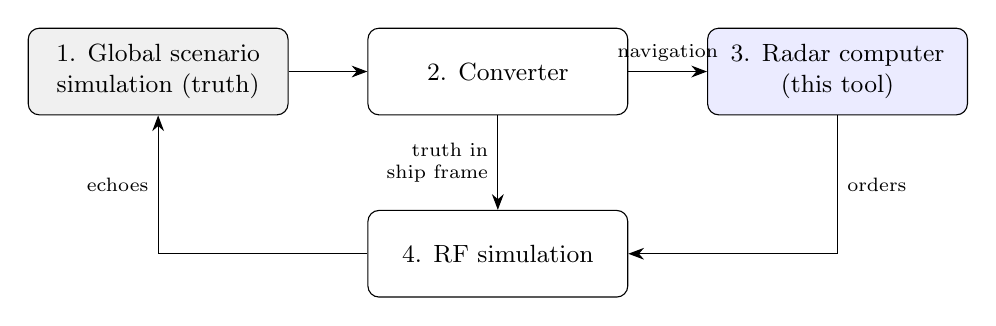
\begin{tikzpicture}[node distance=6mm and 10mm, box/.style={draw,rounded corners,align=center,minimum width=33mm,
  minimum height=11mm,font=\small}, >={Stealth[length=2mm]}]
\node[box,fill=gray!12] (sim) {1. Global scenario\\simulation (truth)};
\node[box,right=of sim] (conv) {2. Converter};
\node[box,right=of conv,fill=blue!8] (rc) {3. Radar computer\\(this tool)};
\node[box,below=12mm of conv] (rf) {4. RF simulation};
\draw[->] (sim) -- (conv);
\draw[->] (conv) -- node[above,font=\scriptsize]{navigation} (rc);
\draw[->] (conv) -- node[left,font=\scriptsize,align=right]{truth in\\ship frame} (rf);
\draw[->] (rc) |- node[pos=0.25,right,font=\scriptsize]{orders} (rf);
\draw[->] (rf.west) -| node[pos=0.75,left,font=\scriptsize]{echoes} ($(sim.south)+(0,0)$);
\end{tikzpicture}
\caption{Four-layer architecture: truth and knowledge are kept apart. The tool implements layer 3 in mission
preparation.}
\label{fig:layers}
\end{figure}

\subsection{Design method}
The model was rebuilt step by step along a roadmap (Section~\ref{sec:roadmap}). A few rules shape every part of it:
\begin{itemize}
  \item \textbf{One parameter file.} Every system value is an entry of \code{radar\_system.toml} with
        \code{value}, \code{unit}, \code{status} (V: locked by the designer; D: derived or proposed, to confirm),
        \code{source} (the reason) and \code{date}. Tool settings (search grids, caches, defaults) are in a separate
        \code{[tool.*]} block. 290 system entries exist today, 247 of them locked.
  \item \textbf{Derived, not entered.} Anything that follows from other values is computed: the array build-up, the
        radiation patterns, the system noise temperature, the converter noise figure, the longest pulse, the
        frequency grid, \dots{} The loader refuses inconsistent combinations with a clear message.
  \item \textbf{Optimistic technology, median threats.} For our technology, the optimistic end of a credible
        2050--2060 range is kept; for threats and the environment, the median or class mean.
  \item \textbf{Approximations by decision only.} Exact shortcuts (closed forms, caches, exact pruning) come first;
        since 25 October 2026 approximations are allowed when they do not denature the model, each one decided by
        the designer with its measured effect and kept as a setting whose exact value stays available.
\end{itemize}

%=====================================================================================================================
\section{The radar}
%=====================================================================================================================

\subsection{Faces and geometry}
The radar has \textbf{four planar faces} spread at \SI{90}{\degree} around the spacecraft axis (azimuths
\SIlist{0;90;180;270}{\degree}), all \textbf{tilted by \SI{25}{\degree} toward the nose}. The ship frame has $Z$
along the axis, toward the nose (``lighthouse'' model: the axis is vertical, the nose at the zenith); azimuth $\varphi$
is counted about $Z$ from $+X$ toward $+Y$, elevation $\varepsilon$ from the $XY$ plane toward $+Z$.

Each face covers a \emph{sector} of radius \SI{75}{\degree} around its normal (the widest scan limit of the bands),
cut by the planes $\varphi = \pm\SI{45}{\degree}$ between neighbouring faces. Search positions are counted in the
direction cosines $(u, v)$ of the face: a planar array scans with a beam of constant width in $(u,v)$, which widens as
$1/\cos\theta$ in angle. The sector covers an area of $2.0006$ in $(u,v)$.

The spacecraft geometry comes from a low-polygon 3D model (\SI{149.46}{m} long, \SI{74.68}{m} span over its radiator
wings, hull diameter \SI{17.22}{m}); the four radar panels are octagons sitting on a cone around the nose station, with
the aperture centres \SI{5.248}{m} from the axis. The loader checks the model against the locked dimensions and checks
that each aperture centre lies on a panel whose normal is the face normal at the locked tilt.

\subsection{Bands and roles}
\begin{center}
\begin{tabularx}{\linewidth}{@{}lLL@{}}
\toprule
 & \textbf{S band} & \textbf{Ku band}\\
\midrule
Usable band & \SIrange{2.60}{2.93}{GHz} & \SIrange{13.5}{14.5}{GHz}\\
Core band (no edge loss) & \SIrange{2.66}{2.88}{GHz} & \SIrange{13.7}{14.3}{GHz}\\
Role & search (detection of new targets) & confirmation of detections, active tracking\\
Scan limit & \SI{75}{\degree} up to \SI{2.85}{GHz}, \SI{70}{\degree} above & \SI{75}{\degree} up to \SI{14.25}{GHz}, \SI{70}{\degree} above\\
TRMs per face & \num{4900} & \num{122500}\\
Peak power per TRM (PA output) & \SI{2000}{W} & \SI{75}{W}\\
Peak power per face & \SI{9.80}{MW} & \SI{9.19}{MW}\\
Instantaneous bandwidth & \SI{200}{MHz} & \SI{200}{MHz}\\
Cold-sky system temperature & \SI{144.5}{K} & \SI{230.8}{K}\\
\bottomrule
\end{tabularx}
\end{center}

The architecture is \textbf{fully digital}: one analogue-to-digital converter per TRM and per polarisation channel,
digital true time delay in every TRM (no beam squint, no aperture-fill limit on the bandwidth), receive beams formed
by computation. Search uses S band only; the S ``touch'' of one confirmation mode is the single exception.

\subsection{Array build-up}
Each face is a dual-band tiling of \textbf{196 TRSAs} (transmit-receive sub-arrays). A TRSA is a square tile of
$25\times25$ Ku TRMs (pitch \SI{10.4}{mm}) and $5\times5$ S TRMs (pitch \SI{52}{mm}, close to $\lambda/2$ in S); each
S TRM covers exactly one block of $5\times5$ Ku TRMs. The TRSAs are laid out in an approximate octagon of 16 centred
rows,
\[
  [6, 8, 10, 12, 14, 16, 16, 16, 16, 16, 16, 14, 12, 10, 8, 6],
\]
separated by a mechanical gap of \SI{0.5}{mm} (a dead, non-radiating region). Derived quantities:
\begin{center}
\begin{tabular}{@{}lr@{}}
\toprule
TRSA side & \SI{260}{mm}\\
Emissive area & \SI{13.2496}{m^2} (fill \SI{99.65}{\percent} of \SI{13.2964}{m^2})\\
Envelope $\Denv$ (widest row: 16 TRSAs and 15 gaps) & \SI{4.1675}{m}\\
Mean element pitch (TRSA pitch / TRMs per side) & S \SI{52.1}{mm}, Ku \SI{10.42}{mm}\\
RMS extent of the aperture along one axis $x_{\mathrm{rms}}$ & \SI{1.033}{m} $= 0.248\,\Denv$\\
\bottomrule
\end{tabular}
\end{center}
The gap was reduced from \SI{2}{mm} to \SI{0.5}{mm} because the break of the element pitch from one TRSA to the next
creates ``gap lobes'' near the grating lobe (\SI{-16.6}{dB} in Ku with \SI{2}{mm}) that no receive weighting can
lower; \SI{0.5}{mm} assumes TRSA and back-plate materials matched in thermal expansion.

\begin{figure}[ht]
\centering
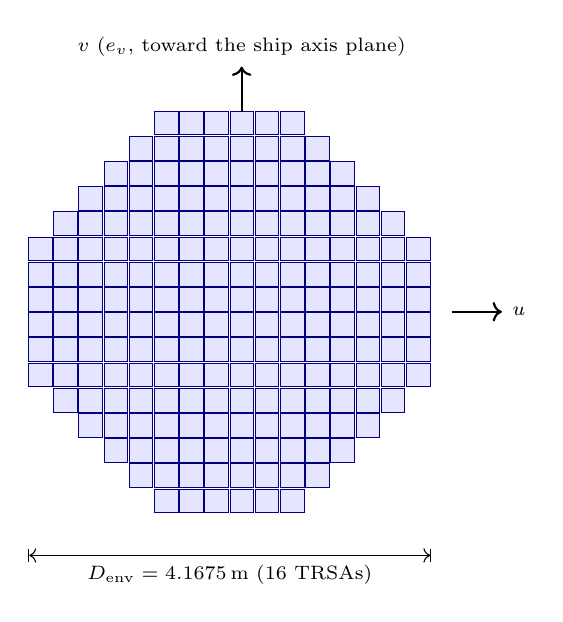
\begin{tikzpicture}[scale=0.32]
  \foreach \n [count=\r from 0] in {6,8,10,12,14,16,16,16,16,16,16,14,12,10,8,6} {
    \pgfmathsetmacro{\xo}{-\n/2}
    \foreach \k in {1,...,\n} {
      \pgfmathsetmacro{\x}{\xo+\k-1}
      \draw[fill=blue!10,draw=blue!50!black,line width=0.2pt] (\x,7.5-\r) rectangle ++(0.94,0.94);
    }
  }
  \draw[->,thick] (0.47,8.4) -- (0.47,10.2) node[above,font=\scriptsize]{$v$ ($e_v$, toward the ship axis plane)};
  \draw[->,thick] (8.8,0.47) -- (10.8,0.47) node[right,font=\scriptsize]{$u$};
  \draw[|<->|] (-8,-9.2) -- (8,-9.2) node[midway,below,font=\scriptsize]{$\Denv = \SI{4.1675}{m}$ (16 TRSAs)};
\end{tikzpicture}
\caption{The 196 TRSAs of one face (each square: $25\times25$ Ku TRMs and $5\times5$ S TRMs).}
\label{fig:octagon}
\end{figure}

%=====================================================================================================================
\section{Antenna model}
%=====================================================================================================================

\subsection{Radiation pattern computed from the build-up}
The pattern is computed from the element positions of the build-up (\code{core/antenna.py}). Elements are isotropic in the array factor; the element pattern enters only through the
projected area $\cos\theta$ and the active mismatch (Section~\ref{sec:mismatch}). Near boresight, expressed in units
of $\lambda/\Denv$, the pattern does not depend on frequency, so one computation per band serves the whole band (S and
Ku sample the same octagon and agree to \SI{0.1}{\percent}). The rows are centred and palindromic, so the array factor
is real,
\[
  AF(u,v) = \sum_{\text{quadrant}} w\,m\,\cos(k x u)\cos(k y v),
\]
with multiplicities $m$ for the symmetry; with the $x\leftrightarrow y$ symmetry of the octagon, cuts from
\SIrange{0}{45}{\degree} suffice, each a matrix product. Results are cached under a hash of their inputs.

\begin{itemize}
  \item \textbf{Transmit beam}: uniform illumination (PAs saturated). Half-power beamwidth (smallest cut)
        $1.036\,\lambda/\Denv$, i.e. \SI{1.525}{\degree} at \SI{2.8}{GHz} and \SI{0.305}{\degree} at \SI{14}{GHz};
        first sidelobe \SI{-15.6}{dB}.
  \item \textbf{Receive beam}: circular Taylor (Hansen) law, $\bar n = 5$, whose design level is \emph{fitted
        numerically} (regula falsi) so that the level \emph{achieved} on the real octagon equals the option chosen for
        the watch volume: \SIlist{-25;-30;-35}{dB}. Efficiency and beamwidth follow:
        \begin{center}
        \begin{tabular}{@{}lccc@{}}
        \toprule
        Option & design level & $\eta_{\mathrm{RX}}$ & HPBW ($\lambda/\Denv$)\\
        \midrule
        \SI{-25}{dB} (default) & \SI{29.5}{dB} & 0.873 & 1.173\\
        \SI{-30}{dB} & \SI{35.7}{dB} & 0.773 & 1.255\\
        \SI{-35}{dB} & \SI{41.7}{dB} & 0.693 & 1.325\\
        \bottomrule
        \end{tabular}
        \end{center}
        Lowering the level rejects strong off-axis sources (bright target, Moon or Earth, jammer) at the cost of receive
        gain ($-0.53$ and $-1.00\dB$ against the \SI{-25}{dB} option). One setting per volume serves S and Ku.
  \item \textbf{Gain}: $G = 4\pi A\,\eta\,\eta_{\mathrm{ohm}}\cos\theta/\lambda^2$ with the emissive area $A$; at
        \SI{2.8}{GHz} on boresight, \SI{41.62}{dBi} in transmission and \SI{41.03}{dBi} in reception (\SI{-25}{dB});
        Ku transmit gain at \SI{14}{GHz}: \SI{55.60}{dBi}.
  \item \textbf{Angle accuracy}: the Cram\'er--Rao bound of the full digital aperture with a margin of 1.13,
        \[ \sigma_u = 1.13\,\frac{\lambda}{2\pi\,x_{\mathrm{rms}}\sqrt{2\,\SNR}}, \]
        independent of the receive weighting (the maximum-likelihood estimator uses the whole aperture); the same
        margin applies to the Doppler and range estimators.
\end{itemize}

\subsection{Far sidelobes and gap lobes}
Beyond the near window ($8\,\lambda/\Denv$), the array factor is scanned on a 2D grid over the whole visible region of
the band (radius $(1+\sin\theta_{\lim})\Denv/\lambda$ at the top of the band), grating-lobe neighbourhoods excluded.
A cumulative profile stores the peak lobe level within a distance $r$ of the beam axis; a lobe at $r$ becomes visible
once the beam is scanned to $\theta$ with $r\lambda/\Denv \le 1+\sin\theta$ (worst azimuth). The strongest far lobes,
gap lobes included, are \SI{-25.3}{dB} in Ku and \SI{-30.7}{dB} in S (uniform); weighting does not lower gap lobes.
For each sector the tool reports up to which scan angle the receive option is held over the visible region; in Ku the
\SIlist{-30;-35}{dB} options are held up to \SIlist{75;62}{\degree} at \SI{14}{GHz} only.

The same module provides \emph{azimuthal means} of the receive power pattern versus the distance to the beam axis
(fine near the axis, annulus means beyond). They are used for the sky-noise integral, the sidelobe clutter and the
jammer pick-up (Sections~\ref{sec:sky} and~\ref{sec:env}). By Parseval's theorem the normalisation is exact: a body
filling the whole front half-space adds its brightness temperature (checked to within 1.00--1.04).

\subsection{Active mismatch and grating lobes}\label{sec:mismatch}
One model, applied to S and Ku, in transmission and in reception, describes the active reflection of the array: a
current sheet matched at $\theta_m = \SI{45}{\degree}$ by a wide-angle impedance-matching (WAIM) layer, and the rise
of the reflection as the first grating lobe approaches the visible region ($g_0 = 0.02$, $d_{\mathrm{mean}}$ the mean
element pitch, worst azimuth):
\begin{align*}
  |\Gamma_{\mathrm{WAIM}}| &= \frac{|\cos\theta - \cos\theta_m|}{\cos\theta + \cos\theta_m},\qquad
  |\Gamma_{\mathrm{GL}}| = \exp(-g/g_0),\quad g = \frac{\lambda}{d_{\mathrm{mean}}} - \sin\theta - 1,\\
  1 - |\Gamma|^2 &= (1 - |\Gamma_{\mathrm{WAIM}}|^2)(1 - |\Gamma_{\mathrm{GL}}|^2),
\end{align*}
with a loss per pass $-10\log_{10}(1-|\Gamma|^2)$, counted twice (transmit and receive). At \SI{2.8}{GHz} the round
trip costs \SI{0.26}{dB} on boresight, 0 at \SI{45}{\degree}, \SI{1.12}{dB} at \SI{70}{\degree} and \SI{2.11}{dB} at
\SI{75}{\degree}. The upper edge of the S band is set by this wall: at \SI{2.93}{GHz} and \SI{70}{\degree} the loss is
\SI{0.97}{dB} per pass; a grating lobe becomes visible at \SI{3.0}{GHz}. The optimiser flags any bin used beyond
\SI{3}{dB} per pass.

The transmit polarisation is linear along $e_v$ (the face axis in the plane of the ship axis), one PA per TRM; its
purity (Ludwig-3 cross-polarisation, $(1+\cos\theta)/(1-\cos\theta)$ in the \SI{45}{\degree} plane) is reported. With
the dual-polarisation receiver it costs nothing in the budget.

\subsection{Sub-apertures for the transmit partition}\label{sec:subap}
For the aperture-partition multibeam mode (Section~\ref{sec:multibeam}) the face is cut into halves (horizontal cut
\code{h}: rows above the centre; vertical cut \code{v}: columns right of the centre) or quadrants, each uniform. Their
2D patterns are evaluated directly (a half is not centred, so no symmetry is assumed), exactly, by a sum separable by
element rows:
\begin{center}
\begin{tabular}{@{}lccc@{}}
\toprule
Aperture & S TRMs & $-3\dB$ widths $u\times v$ ($\lambda/\Denv$) & lattice cell / full face\\
\midrule
Full face & \num{4900} & $1.041\times1.041$ & 1\\
Half & \num{2450} & $1.041\times1.928$ & $\times1.85$\\
Quadrant & \num{1225} & $1.928\times1.928$ & $\times3.43$\\
\bottomrule
\end{tabular}
\end{center}
The cell ratio is below 2 and 4 because half an octagon is not half as wide in effective width. Because the octagon is
symmetric in $x$ and $y$, the two halves are the same beam rotated by \SI{90}{\degree}: the code checks this exactly
and then searches only one of them.

%=====================================================================================================================
\section{Transmit chain and power budget}
%=====================================================================================================================

\subsection{TRM model}
The TRMs are GaN-on-diamond with micro-channel cooling. Peak power is specified at the PA output (where the
power-added efficiency, PAE, is defined); the path from the PA to the element is a derived loss (harmonic filter,
circulator, calibration coupler, line: \SI{0.6}{dB} in S, \SI{0.95}{dB} in Ku).

\paragraph{PAE.} For a pulse of length $\tau$ in a train of duty cycle $d = \tau/\mathrm{PRI}$,
\[
  \eta = \eta_{\mathrm{sat}}\,\frac{\tau}{\tau + t_{\mathrm{edge}}}\,\min\bigl(1,\;1 - a\,(d - d_{\mathrm{ref}})\bigr),
\]
with the saturated PAE $\eta_{\mathrm{sat}}$ at the reference duty $d_{\mathrm{ref}} = 0.10$, the time $t_{\mathrm{edge}}$
during which the PA draws power without full RF (switching, bias and phase settling), and a slope $a$ for channel
heating. A single pulse uses $d_{\mathrm{ref}}$.

\begin{center}
\begin{tabular}{@{}lcc@{}}
\toprule
 & S & Ku\\
\midrule
$\eta_{\mathrm{sat}}$ & 0.80 & 0.65\\
$t_{\mathrm{edge}}$ & \SI{0.2}{\micro s} & \SI{0.1}{\micro s}\\
Duty slope $a$ & 0.05 ($-2.75\,\%$ at $d=0.65$) & 0.08 ($-4.4\,\%$ at $d=0.65$)\\
Duty ceiling on trains & 0.65 & 0.65\\
Energy buffer per TRM & \SI{25}{J} & \SI{1.2}{J}\\
Longest pulse $\tau_{\max}$ & \SI{2.0}{ms} & \SI{2.08}{ms}\\
\bottomrule
\end{tabular}
\end{center}

\paragraph{Energy buffer.} Each TRM draws its pulse from a local capacitor bank. A pulse using a fraction
$x = E/E_{\mathrm{buf}}$ of it loses on average $-10\log_{10}(1-x/2)$ (the PA output follows the stored energy); a
pulse beyond $x = 0.2$ is refused, which sets
$\tau_{\max} = 0.2\,E_{\mathrm{buf}}\,\eta_{\mathrm{sat}}/P_{\mathrm{pk}} - t_{\mathrm{edge}}$. The longest pulse ends
\SI{0.97}{dB} down (mean \SI{0.46}{dB}); the AM/PM conversion of the PA as the buffer empties is reported, not
counted (quasi-linear phase drift).

\subsection{Electrical budget}\label{sec:power}
The budget of a face is \emph{electrical}: every look costs its RF energy divided by the PAE of its pulse, and the heat
of the face is the electrical energy minus the RF energy (about \SI{370}{W} per S TRM during a long train at
$d = 0.65$, an input of the thermal step). Since roadmap step 4.1 the electrical power is modelled at four levels.

\paragraph{Ship level: a shared budget.} The spacecraft provides \SI{8}{MW} to the radar. The faces do \emph{not} have
fixed shares: they draw from this budget in common, so a heavily loaded face may take more than a quarter when the
others need less. The verdict on energy is therefore taken for the ship,
\[
  \sum_{k=1}^{4} P_{\mathrm{bus},k} \le \SI{8}{MW},\qquad
  P_{\mathrm{bus},k} = \frac{P_{\mathrm{TX},k} + P_{\mathrm{on}} + p_{\mathrm{pump}}\,Q_k}{\eta_{\mathrm{psu}}\,\eta_{\mathrm{dist}}},
\]
where $P_{\mathrm{TX},k}$ is the mean electrical power of the transmissions of face $k$ (search, confirmation,
tracking, at the TRM supply), $P_{\mathrm{on}}$ the always-on consumption, $Q_k$ the mean heat of the face and
$p_{\mathrm{pump}} = 2\,\%$ the share of that heat spent by the cooling pumps; $\eta_{\mathrm{psu}} = 0.95$ and
$\eta_{\mathrm{dist}} = 0.995$ are the efficiencies of the power supply and of the distribution (product 0.945). Each
face is also limited by what its own feeder (cables, converter) can carry, \SI{8}{MW}, and by an optional cap the
operator may reserve for it in the mission (one value for all faces or one per face). The tool reports the power each
face actually draws, the margin left in the shared budget and the split among the faces (Section~\ref{sec:load}). To
weigh energy against time when it chooses waveforms, the search optimiser keeps a \emph{reference} allocation of
$\SI{8}{MW}/4 = \SI{2}{MW}$ per face.

\paragraph{Always-on consumption.} A digital array receives all the time, whether it transmits or not. Per face:
two converters per TRM (one per polarisation; \SI{0.1}{W} each at \SI{250}{MS/s} and 13 bits, an optimistic 2050 value
against 0.3--1 W today) and two receive chains per TRM (LNA, amplifiers, local-oscillator distribution: \SI{0.5}{W}
in S, \SI{0.1}{W} in Ku), in both bands; \SI{50}{kW} of digital beamforming and processing (ceiling,
Section~\ref{sec:compute}); \SI{2}{kW} of control. Total \SI{106.9}{kW} per face (\num{9800} S and \num{245000} Ku converters).
With the reference \SI{2}{MW}, a face has $2\times0.945 - 0.107 = \SI{1.784}{MW}$ left for its transmissions.

\paragraph{TRM level: supply over a train.} Each TRM draws its pulse from its local buffer and refills it from a
continuous supply (\SI{1700}{W} in S, \SI{80}{W} in Ku). Over a train of $n$ pulses of energy
$E_p = P_{\mathrm{pk}}\tau/\eta$ every PRI, two conditions must hold: the mean power $E_p/\mathrm{PRI}$ stays within the
supply, and the buffer, recharged at the supply rate between pulses, loses at most the allowed fraction:
\[
  (n-1)\,\max\bigl(0,\;E_p - P_{\mathrm{sup}}\,\mathrm{PRI}\bigr) + E_p \le 0.2\,E_{\mathrm{buf}}.
\]
A waveform that breaks either condition is removed from the search spaces (no S waveform today; 68 of \num{2356} Ku
looks, long trains at high duty).

\paragraph{Face level: storage and peak power.} While a face transmits, all its TRMs draw together: about
\SI{12.3}{MW} for a full-power S look ($\num{4900}\times\SI{2}{kW}/0.8$) and \SI{14.1}{MW} in Ku, far above the mean
the bus delivers. The difference comes from an energy storage per face (supercapacitors, \SI{5}{MJ}, \SI{80}{\percent}
usable, \SI{15}{MW} discharge), recharged at the rate the feeder leaves after the always-on consumption. Three checks:
\begin{itemize}
  \item \emph{one observation}: the energy of the costliest observation of the plan (an S search dwell or a Ku look),
        minus the recharge during it, must fit in the usable storage;
  \item \emph{worst burst}: if all the transmissions of the longest revisit of the face were packed together, the
        deficit $RR\,(P_{\mathrm{TX}} - P_{\mathrm{rech}}\,f_t)$ ($f_t$ the share of time on air) must fit in the usable
        storage; it never does for long revisits, so this check yields a \emph{scheduler rule}: at most
        $E_{\mathrm{usable}}/(P_{\mathrm{peak}} - P_{\mathrm{rech}})$ of contiguous transmission at peak power (about
        \SI{0.3}{s}), then recharge;
  \item \emph{peak power}: the peak of an observation must stay within the storage discharge plus the recharge.
\end{itemize}
The step of the bus load at the start of an observation and its slope over the pulse edge (\SI{0.2}{\micro s} in S)
are reported for the design of the bus.

\subsection{Thermal budget}\label{sec:thermal}
All the electrical power a face draws becomes heat, except the RF energy radiated away. Since roadmap step 4.2 the
heat is checked at three scales, each with its own time constant.

\paragraph{Coolant and cold plate.} Each face is cooled by micro-channels in its cold plate, with a dielectric coolant
(a derivative of the submer SmartCoolant; 2020 values: heat capacity \SI{2.26}{kJ/(kg.K)}, heat-transfer coefficient
about \SI{2050}{W/(m^2.K)} pumped, density 0.796). Assumed for 2050--2060: \SI{2.5}{kJ/(kg.K)},
\SI{3000}{W/(m^2.K)}, 0.8. The micro-channels wet ten times the footprint; the plate may run \SI{40}{K} above a
\SI{20}{\celsius} coolant. Hence an admissible heat flux of $h \times 10 \times \SI{40}{K} = \SI{120}{W/cm^2}$ and a
cooling capacity of about \SI{15.9}{MW} per face: far above what a face dissipates (a TRM in a long S train releases
about \SI{14}{W/cm^2} over its footprint; a face drawing the whole \SI{8}{MW} dissipates about \SI{2}{MW}). All these
figures are derived from the file, so a change of the coolant specification is absorbed.

\paragraph{Heat of a face.} The loop of a face carries the heat of the transmissions (electrical minus RF energy), the
always-on electronics (\SI{106.9}{kW}) and the pumps; the losses of the power conversion go to the ship. A burst of
transmissions is absorbed by the thermal inertia of the face (\SI{50}{L} of coolant and about \SI{100}{kg} of
structure, \SI{190}{kJ/K}; \SI{10}{K} of admissible rise, a buffer of \SI{1.9}{MJ}); the tool checks the worst burst
and gives the longest contiguous transmission at peak heat as a scheduler rule (none is needed today).

\paragraph{Junction of the power amplifiers.} The junction temperature of a TRM amplifier follows a two-pole Foster
network (die and diamond spreader: S \SI{0.02}{K/W} at \SI{10}{\micro s} and \SI{0.03}{K/W} at \SI{1}{ms}; Ku
\SI{0.2}{K/W} and \SI{0.3}{K/W}) driven by the heat of each pulse, plus the convection to the coolant at the mean heat.
Over every search waveform and Ku look it stays below \SI{63}{\celsius}, far from the \SI{225}{\celsius} limit, even in
continuous transmission: thermal heating does not limit the duty cycle, whose ceiling of 0.65 stands for the efficiency
and supply limits. The temperature is reported per waveform; the removal of waveforms above the limit exists as a
setting and is off.

\paragraph{Ship.} The heat of the four faces plus the conversion losses must fit in the heat rejection the spacecraft
reserves for the radar, shared by the faces like the electrical budget (\SI{6}{MW}, provisional).

%=====================================================================================================================
\section{Band model}
%=====================================================================================================================
Each band has a usable band and a core band. A signal of bandwidth $B$ at centre $f$ occupies
$[f-B/2,\,f+B/2]$, which must lie inside the usable band (and outside the spectrum the mission forbids); otherwise the
waveform is not playable at $f$. Outside the core band, a raised-cosine derating reaches \texttt{edge\_derating\_db} at
the usable edges (\SI{1.0}{dB} round trip in S, \SI{0.5}{dB} in Ku); its \emph{exact} average over the occupied
spectrum is applied. The loader checks that the core band and the scan-limit break frequency lie inside the usable
band, so the band can be changed in the file alone. With digital true time delay there is no aperture-fill limit
(phase steering would limit the signal to $c/(\Denv\sin\theta)$, about \SI{75}{MHz} at \SI{75}{\degree}).

%=====================================================================================================================
\section{Receive chain}\label{sec:rx}
%=====================================================================================================================

\subsection{System noise temperature}
$\Tsys$ is the Friis cascade referred to the antenna port: cold-sky antenna temperature, the losses before the LNA
(circulator, limiter, line: they attenuate and add $(L-1)T_{\mathrm{phys}}$), the LNA, the post-LNA chain and the ADC,
each divided by the gain ahead of it, and a digital-noise factor. Values (S / Ku): cold sky \SI{3.2}{K} / \SI{2.8}{K},
front-end at \SI{320}{K}, pre-LNA losses \SI{0.85}{dB} / \SI{1.2}{dB}, LNA noise figure \SI{0.75}{dB} / \SI{1.15}{dB},
giving \textbf{\SI{144.5}{K} in S and \SI{230.8}{K} in Ku} for the cold sky. The sky in front of the face is added per
direction (Section~\ref{sec:sky}).

\subsection{Converter and dynamic range}
The ADC noise figure is derived from the converter:
\[
  \mathrm{NF}_{\mathrm{ADC}} = P_{\mathrm{FS}} - (6.02\,\mathrm{ENOB} + 1.76) - 10\log_{10}(k T_0 f_s),
\]
with 13 effective bits, a full scale of \SI{+10}{dBm} and $f_s = 1.25\times\SI{200}{MHz} = \SI{250}{MS/s}$
complex: \SI{20.0}{dB}. Levels are referred to the antenna port: the clipping level is $P_{\mathrm{FS}} - \SI{3}{dB}$
minus the gain to the ADC (\SI{53.4}{dB} above the noise in S). Digitisation happens per element, \emph{before}
beamforming: a strong source in any front direction reaches every converter. The \emph{minimum unsaturated range} is
where the peak echo per element of a full-power, single-beam look reaches the clipping level (S: \SI{12.2}{km} for
the reference target, \SI{2.3}{km} for a KKV). The receiver is deaf for $\tau$ plus the limiter recovery
(\SI{50}{ns} in S, \SI{25}{ns} in Ku).

\subsection{Dual polarisation}
Each TRM has two receive channels. A detection look uses a GLRT detector on the unknown polarisation of the echo,
estimated over the look: one more unknown complex sample, a loss $\SNR_{\mathrm{req}}(n+1)-\SNR_{\mathrm{req}}(n)$
(\SI{0.47}{dB} for one coherent sample, small for long noncoherent trains). A tracking look knows the polarisation
from the track (\SI{0.05}{dB} residual). The dual-channel receiver also collects the cross-polar echo of the target,
a gain $10\log_{10}(1+\rho)$ with $\rho$ the cross/co-polar RCS ratio, and the two channels add polarisation diversity
to the target fluctuation (Section~\ref{sec:targets}).

\subsection{Isolation between bands and faces}
Leakage from each transmitting band and face to each receiving element is checked against three limits: LNA blocking,
ADC clipping and in-channel desensitisation (\SI{6}{dB} below the noise). With the couplings assumed (\SI{90}{dB} to
an adjacent face, \SI{120}{dB} to the opposite one, \SI{-30}{dB} inside a TRSA) a face cannot receive a band while
another face transmits it: all faces share \textbf{a common transmit/receive cadence per band}. A further rule: no Ku
reception on a face during an S transmission whose fifth harmonic $[5(f-B/2),\,5(f+B/2)]$ covers the Ku channel. These
are rules of the scheduler (Section~\ref{sec:sched}).

\subsection{Sky noise}\label{sec:sky}
The antenna temperature depends on the look direction. With the receive gain written $G = G_0\,w\,g(\rho)$ (element
pattern $w=\cos\theta$, nothing behind the face) and $d\Omega = du\,dv/w$, the factor $w$ cancels and the rise is
\[
  \Delta T = T_b\,\frac{A\,\eta_{\mathrm{RX}}\,\eta_{\mathrm{ohm}}}{\Denv^2}\int_{\text{body}} g(\rho)\,d\rho^2,
\]
the integral running over the body as seen in the $(u,v)$ plane of the face (front half only), $\rho$ being the
distance to the beam axis in $\lambda/\Denv$ and $g$ the azimuthal mean of the computed receive pattern, main lobe
included. Small bodies (Sun, Moon) are sampled finely on their disk; large
ones (Earth) by a polar grid in the near window and rings beyond. Brightness temperatures are class values per band
(quiet, mid-cycle and active Sun: \SIlist{4.5e4;1.0e5;1.5e5}{K} in S; Earth \SI{290}{K} worst case, ocean and land
variants; Moon \SI{230}{K}); the galactic background follows a plane-and-bulge model scaled as $f^{-2.5}$, with a
worst case applied everywhere when the mission gives no galactic frame. The Sun in the beam adds about
\SI{17}{dB} in S as in Ku; the Moon about \SI{2.6}{dB} in Ku.

For a sector, $\Tsys$ is evaluated every half transmit beamwidth over the scanned positions (raster of
\SI{0.2}{\degree}). Near hot sources the noise varies faster than that step, so the raster cells are evaluated one by
one where the rise of their block exceeds \SI{0.5}{dB}, and within three transmit beamwidths of a stand-off jammer,
of a small body's centre or of a large body's limb; each such cell is then split into $8\times8$ points of equal
weight. A point whose rise exceeds \SI{10}{dB} is \emph{blinded}: the cell is searched only for the share of its
points left, and the blinded share is reported with the body responsible. The \emph{budget} $\Tsys$ of the sector is
the $(1-\text{\code{short\_tol}})$ quantile (\SI{99}{\percent}) of the positions not blinded, every point counting
for its own weight, and all its ranges scale with $(T_{\mathrm{cold}}/T_{\mathrm{budget}})^{1/4}$. Turning the sky and
the sector together about the ship axis by angles off the raster moves the budget and the blinded share by less than
\SI{1}{\percent} (Sun, \SI{0.37}{\degree} and \SI{1.13}{\degree}); a steady drift at larger angles (\SI{1.4}{\percent}
at \SI{2.9}{\degree}), believed to come from the fixed faces, is still to be confirmed. The same rule applies in Ku to
the confirmation and tracking of the sector.

%=====================================================================================================================
\section{Waveforms}\label{sec:wf}
%=====================================================================================================================

\subsection{Modulation and pulse compression}
Two families are modelled: linear FM (Doppler tolerant) and non-linear FM (low range sidelobes shaped by the frequency
law, no weighting loss). Phase codes are excluded: poor Doppler tolerance at closing speeds up to \SI{25}{km/s}
($f_d \approx \SI{470}{kHz}$ in S). For each look, with $f_{d,\max} = 2v/\lambda$:
\begin{itemize}
  \item if $f_{d,\max}/B \le 2\,\%$: NLFM, mismatch loss \SI{0.1}{dB};
  \item otherwise: LFM with a Taylor ($\bar n = 5$) receive-only weighting at the sidelobe level of the volume; loss =
        weighting loss $-\,20\log_{10}(1-f_d/B)$ (Doppler loss at the peak of the ambiguity function).
\end{itemize}
The range sidelobe level is the same as the angular option of the volume: one sidelobe policy per volume. Weighting
at \SIlist{-25;-30;-35}{dB} costs \SIlist{0.41;0.68;0.93}{dB} and widens the main lobe by $\times$1.18, 1.27, 1.34.
The physical range resolution is this widening times $c/2B$ (2 m requires \SI{89}{MHz} at \SI{-25}{dB}); the range
estimator constant is $k_r = 0.6/(\text{RMS-bandwidth ratio})$. The range--Doppler coupling bias $c f_d \tau/2B$ is
corrected by the Doppler measurement.

\subsection{Intra-pulse effects and timeline}
A target crosses $n_c = 2v\tau B/c$ range cells during the pulse; a filter matched to another speed then has a
quadratic phase error, a loss $-20\log_{10}\bigl|\langle e^{\,j2\pi n_c x^2}\rangle_{x\in[-1/2,1/2]}\bigr|$ (1 dB at
$n_c = 1.016$). This sets the spacing of the velocity bank (Section~\ref{sec:proc}).

The receiver is deaf during the pulse and the limiter recovery: blind range $c(\tau + t_{\mathrm{rec}})/2$ (\SI{3}{km}
for \SI{20}{\micro s}, \SI{300}{km} for \SI{2}{ms}), which must stay below the sector's shortest range of interest
(\code{range\_min\_km}, 10\,\% of the required range by default). A train is unambiguous in range when
$\mathrm{PRI} \ge 2R/c + \tau + t_{\mathrm{rec}}$; a sector may allow ambiguous trains, staggered over 3 PRIs at
$\pm10\,\%$, with the mean eclipsing loss $-10\log_{10}(1-(\tau+t_{\mathrm{rec}})/\mathrm{PRI})$ (they are removed when
a surface is in the main lobe, since its clutter would fold onto the targets).

\subsection{Frequency agility}
A noncoherent train may hop its carrier pulse to pulse over an excursion $\Delta f$; the occupied band becomes
$B + \Delta f$ and the number of independent target samples is $\min(n, \lfloor \Delta f/(c/2L)\rfloor + 1)$ for a
target of length $L$, which turns a declared Swerling~1/3 target into a 2/4-like one over the train.

\subsection{Transmit multibeam}\label{sec:multibeam}
In S, one dwell may serve $B_{\mathrm{tx}}$ beams. The digital receiver already forms many receive beams per position
(no loss; a computing load). Three transmit modes are modelled:
\begin{itemize}
  \item \textbf{Phase-only superposition} ($B_{\mathrm{tx}} = 2, 4, 8$): every TRM sends the constant-envelope sum of the
        beams (PAs saturated, PAE unchanged), power $P/B_{\mathrm{tx}}$ per beam, full transmit gain, a loss of
        \SIlist{0.4;0.6;0.8}{dB} (power lost to the intermodulation of the constant-envelope sum).
  \item \textbf{Aperture partition} ($B_{\mathrm{tx}} = 2, 4$): halves or quadrants (Section~\ref{sec:subap}), power
        $P/B_{\mathrm{tx}}$ and gain $G\,N_{\mathrm{sub}}/N$ per beam, a wider beam on its own lattice: fewer positions.
  \item \textbf{Time multiplex} ($B_{\mathrm{tx}} = 2, 4, 8$): full-power pulses sent back to back in the PRI; blind
        range, buffer, duty and PAE computed on $B_{\mathrm{tx}}\tau$. Not offered to the optimiser: with interleaved
        positions it spends the same energy and time per position as one beam.
\end{itemize}

\subsection{Search waveform space}
The S search space is the product of: integration (coherent, noncoherent), transmit mode and beams, signal bandwidths
\SIlist{10;20;30;50;75;100;150;200}{MHz} meeting the sector's resolution, pulses from \SI{5}{\micro s} to \SI{2}{ms}
(13 values, the last one set by the buffer), 1 to 32 pulses, the agile variant of noncoherent trains and, where a
surface clutters the sector, Taylor Doppler weightings of coherent trains. The PRI is the shortest unambiguous one
(or \SI{1}{ms} for single pulses and allowed ambiguous trains). About \num{6500} candidates per sector.

%=====================================================================================================================
\section{Signal processing}\label{sec:proc}
%=====================================================================================================================

\subsection{Coherent blocks and coherence}
A coherent train of $N$ pulses is cut into $M$ blocks ($M$ divides $N$) integrated noncoherently, $M$ minimising the
required SNR of $M$ blocks plus the coherence loss of one block. Noncoherent trains, and declared Swerling~2/4 cases,
have $M = N$. The coherence loss of a block of duration $T$ combines
\begin{itemize}
  \item the target decorrelation $\eta = \exp(-(T/T_0)^2)$, with $T_0 = \lambda/(2L\omega)$ from the target class
        (length $L$, rotation rate $\omega$);
  \item the residual phase variance $\sigma^2$, giving $4.34\,\sigma^2\dB$: oscillator phase noise filtered by the
        round trip, $4\sin^2(\pi f\tau_{rt})$, integrated from $1/T$ to $B/2$ (one oscillator for transmit and receive;
        an optimistic photonic oscillator, \SI{-150}{dBc/Hz} at \SI{1}{kHz} from \SI{10}{GHz}), plus the residual
        platform motion $(4\pi\delta/\lambda)^2$ with $\delta = \SI{10}{\micro m}$ rms.
\end{itemize}
The losses are negligible with these values; the visible effect is the Doppler floor, reported per look.

\subsection{Velocity and acceleration banks}
Range migration is compensated (keystone or Radon type, residual \SI{0.1}{dB} when the target crosses more than 1.5
cells). The filter for a velocity offset $\Delta v$ loses the intra-pulse term plus the range walk over the look; the
bank step is chosen so that a target half a step off loses \SI{1}{dB}; the \emph{mean} loss over the step goes into the
budget and the number of hypotheses into the false-alarm count (and, later, the computing load). Accelerations up to
the class maximum add a quadratic phase on a coherent block and a residual range curvature; when they cost more than
\SI{1}{dB}, a bank of acceleration hypotheses multiplies the velocity hypotheses.

\subsection{Grids, CFAR and false alarms}
The detection grid is oversampled $\times4$ in range and the Doppler transform zero-padded $\times4$: mean straddle
\SI{0.05}{dB} and \SI{0.07}{dB}. The CA-CFAR uses \num{1024} reference cells (loss \SI{0.04}{dB}, exact for
Swerling~1 on one sample); OS-CFAR (rank 0.75) and GO-CFAR (greatest of the two half windows, which holds the
$\Pfa$ at a clutter edge, \SI{0.05}{dB}) are options. Independent cells per position: range extent over $c/2B$,
Doppler cells of a block, velocity and acceleration hypotheses, and angular cells (receive beams per position $\times$
the receive-beam spacing squared). The oversampled grids are not counted (correlated samples).

%=====================================================================================================================
\section{Detection criterion}\label{sec:det}
%=====================================================================================================================

\subsection{Exact detection laws}
A square-law detector on $n$ noncoherently integrated samples (the coherent blocks) is modelled exactly: under noise
alone the statistic is Gamma$(n,1)$, so $\Pfa = P(\mathrm{Poisson}(T) \le n-1)$; for a steady target of total SNR
$\lambda$, $\Pd = \sum_k \mathrm{Pois}(k;\lambda)\,P(\mathrm{Poisson}(T)\le n+k-1)$. Fluctuating targets are mixtures
over a Gamma-distributed target power of shape $k$ ($k=1$: Swerling~1, $2$: Swerling~3, $n$: Swerling~2, $2n$:
Swerling~4, $\infty$: steady); non-integer shapes are allowed, which is how decorrelation inside a look and
polarisation diversity enter. The laws are valid for any $\Pfa$ and agree with Shnidman's fit within its
\SI{0.3}{dB} error.

\subsection{Pd averaged over the target position}
The random position of the target costs SNR. The offsets in the hexagonal transmit cell (real pattern), in the receive
beam lattice, in range and Doppler straddle, and to the nearest velocity filter form a discrete loss law (16 quantiles
each, combined as independent). The $\Pd$ of a look is the \emph{mean} $\Pd$ over this law, and the SNR it costs is
the budget loss called ``positions''. A spacing of $1.4$ transmit beamwidths is the optimum of this criterion for
one look (flat within \SI{0.1}{dB} from 1.3 to 1.6); since the cumulative criterion lowers the $\Pd$ asked of a look,
the optimiser chooses the spacing of each sector among 1.3 to 2.0 by steps of 0.1 (Section~\ref{sec:opt}). A cell
corner is \SI{7.9}{dB} down at 1.4, so the scheduler must shift the lattice every frame.

\subsection{Cumulative Pd of the search}
A target closing at $v$ is seen once per revisit $RR$, at ranges $R(1+(k+\phi)q)$ with $q = vRR/R$ and a uniform phase
$\phi$; the look SNR scales as $(R/R_k)^4$. The requirement is that the \emph{cumulative} probability
\[
  P_{\mathrm{cum}}(R) = \bigl\langle 1 - \textstyle\prod_k (1 - P_{\mathrm{d},k})\bigr\rangle_\phi = 0.9
\]
at the sector's required range (looks below $\Pd = 10^{-3}$ no longer count). Against a single look at $R$ this changes
the required SNR by $+6.0\dB$ for $q=1$ and $-6.8\dB$ for $q=0.1$.

\subsection{False-alarm policy}
By default a sector tolerates a number of false alarms per revisit (\code{fa\_per\_rr} = 10); the $\Pfa$ per cell is
that number divided by positions times independent cells, bounded to $[10^{-14}, 10^{-4}]$ and rounded to a twentieth
of a decade. Every false alarm is then confirmed in Ku like a detection. Ku looks use $\Pfa = 10^{-8}$.

%=====================================================================================================================
\section{Target models}\label{sec:targets}
%=====================================================================================================================
Targets are described by \emph{classes} whose values are \emph{class means} (the adversary's equipment is unknown). A sector names a class and may
override any value. ST is the conventional reference target of the benchmark; GENERIC completes a sector that names no
class.

\begin{center}
{\small\setlength{\tabcolsep}{4pt}\begin{tabular}{@{}lcccccccc@{}}
\toprule
Class & $v$ (km/s) & $L$ (m) & $\omega$ (\si{\degree/s}) & $a_{\max}$ & RCS S / Ku (\si{m^2}) & Fluct. & Depol. & $T_0$ S / Ku (s)\\
\midrule
ST (reference) & 5 & 10 & 0.1 & 0 & \num{1000} / \num{1000} & SW1/2 & \SI{-10}{dB} & 3.1 / 0.6\\
GENERIC & 10 & 3 & 1 & 1\,g & 1 / 1 & SW1/2 & \SI{-10}{dB} & 1.0 / 0.20\\
KKV & 25 & 1.5 & 1 & 10\,g & 1.27 / 13.8 & SW3/4 & \SI{-20}{dB} & 2.0 / 0.41\\
SHIP & 5 & 100 & 0.1 & 1\,g & 300 / 300 & SW1/2 & \SI{-6}{dB} & 0.31 / 0.06\\
DEBRIS & 15 & 0.5 & 10 & 0 & 0.01 / 0.01 & SW1/2 & \SI{-3}{dB} & 0.61 / 0.12\\
DECOY & 25 & 1.5 & 0.5 & 0 & 0.135 / 0.135 & SW0 & \SI{-20}{dB} & 4.1 / 0.82\\
\bottomrule
\end{tabular}}
\end{center}

\paragraph{Frontal RCS and seeker optics.} The RCS is co-polar and frontal (the aspect of a closing target). The KKV
front is a large infrared seeker mirror, metallic and therefore a perfect conductor at radar frequencies, pointed at
its target. Its contribution is
$\sigma_{\mathrm{opt}} = \max\bigl(\pi(2f)^2,\;\eta_r\,4\pi A^2/\lambda^2\bigr)$ with $A = \pi D^2/4$, $D = \SI{0.3}{m}$,
$f/D = 1$, $\eta_r = 0.1$: direct reflection on the concave primary, and the ``cat's eye'' retro-reflection of the
focal assembly, in $1/\lambda^2$, hence mostly in Ku. The decoy mimics the body without the optics, which will help
discrimination.

\paragraph{Fluctuation.} The fluctuation of a look is a Gamma shape: the family (SW1/2: one degree of freedom per
independent sample, SW3/4: two, SW0: steady) times $\min(n, 1 + T_{\mathrm{obs}}/T_0)$ independent samples over the
look ($n$ coherent blocks), times the polarisation diversity $(1+\rho)^2/(1+\rho^2)$ of the two receive channels.
A declared Swerling case overrides the class.

\paragraph{Masking.} The scene is unknown, so the masking of a weak target by a strong neighbour is an output: the
envelope of the strong target's response at 1, 2 and 3 cells in range (with the look's weighting) and Doppler
(\SI{-13.3}{dB} beyond one cell without a Doppler window).

%=====================================================================================================================
\section{Environment}\label{sec:env}
%=====================================================================================================================

\subsection{Spacecraft structure}
The obstacles are in the near field of the aperture (Fraunhofer limit about \SI{325}{m} in S): the beam is a tube of
the width of the aperture. Rays are cast from 37 points of the aperture along the pointing direction, exactly on the
triangles of the 3D model; the blocked fraction $f$ costs $-20\log_{10}(1-f)$ per pass, and a position beyond
\SI{3}{dB} per pass is masked. The structure also radiates: its emissivity times physical temperature (hull
$\varepsilon = 0.01$ at \SI{290}{K}, radiators $0.05$ at \SI{750}{K}) is picked up by the main lobe through the
blocked fraction and by the far sidelobes as a body of the sky. With the \SI{25}{\degree} tilt, the structure only
blocks directions more than \SI{71.7}{\degree} from a face normal, all served by another face at a smaller scan: no
position is masked and the radiators are never seen; the hull adds a negligible \SI{2.9}{K}.

\subsection{Surfaces: shadow, clutter, converter saturation}
Bodies with a surface (Earth, Moon) are spheres at a distance $D$ given by their angular radius. A direction inside the
disk meets the surface at $d = D\cos\delta - \sqrt{R^2 - D^2\sin^2\delta}$; nothing exists beyond. The surface
backscatter is ``constant-$\gamma$'', $\sigma_0 = \gamma\cos\theta_i$ ($\gamma$ = radar albedo; Earth \SI{-12}{dB} in
S, Moon \SI{-11.5}{dB}). The sidelobe clutter in the target's range cell $r$ comes from the iso-range ring of the
surface (area $2\pi R r\,\Delta r/D$ per cell), sampled on 720 points and seen through the two-way pattern:
$y = \sigma_c/\sigma_{\mathrm{target}}$. The main-lobe echo of a surface is checked against the ADC clipping level per
element (alert), and a limb inside a sector is flagged (GO-CFAR advised there).

\subsection{Clutter per waveform}\label{sec:clutter}
In S, the clutter is evaluated \emph{per candidate waveform and per \SI{1}{\degree} scan bin}, out of the $\Tsys$
budget (Ku keeps a simpler noise-factor model until its own step):
\begin{itemize}
  \item \textbf{Clutter ratio} $y$, per pointing and per transmit beam of the search space (full face, or the 2D
        pattern of a partition sub-aperture), at the requirement range of the pointing, for a reference range cell;
        it scales exactly as $c/2B$ with the candidate's bandwidth, and is divided by the number of coherent blocks
        $M$ (the per-block requirement).
  \item \textbf{Doppler residual} $\rho(v)$: the surface's Doppler spectrum (Gaussian, mean and 1-$\sigma$ spread of
        its closing speed given by the scenario), folded over the PRF, through the filter of a coherent block
        (uniform weights $w_k$, or Taylor \SIlist{-30;-40}{dB}),
        \[ H(x) = \Bigl|\textstyle\sum_k w_k e^{j2\pi kx}\Bigr|^2 \big/ \bigl(\textstyle\sum_k w_k\bigr)^2, \]
        plus a white floor from the residual phase variance through the filter's noise bandwidth. $\rho = 1$ without
        coherent blocks or without the scenario's closing speed (prudent). It is evaluated at 11 target speeds over the
        sector's span.
  \item \textbf{Range}: clutter is treated as noise at the detector, $S/(N + C)$ with $C/N = a\,S/N$,
        $a = y\,\rho(v)/M$. In each bin $y$ is taken at the 99\,\% quantile of the pointings; the SNR increase $G$ that
        restores the look's $\Pd$ \emph{averaged over the target speeds} is solved by bisection, and the range becomes
        $R_n G^{-1/4}$. If no power restores it, the candidate is unplayable in the bin; a pointing that no candidate
        can clear is blinded.
  \item \textbf{Requirement brought back to the surface}: where a pointing meets a surface at $d$ below the required
        range, the requirement becomes $d - \text{guard}$ (guard = max(\SI{10}{km}, range resolution)), rounded
        \emph{up} on a grid of 5\,\% of the range; the cumulative criterion is recomputed for each such class; with
        $d - \text{guard} \le 0$ there is no volume and the pointing is not scanned.
\end{itemize}

\subsection{Jammers}
\paragraph{Stand-off jammers} are declared in the sky. Their noise enters $\Tsys$ through the receive pattern:
$T_j = (\text{EIRP density}/4\pi R^2)/k \times A_{\mathrm{eff}}(\text{direction})$. A jammer more than one receive
beamwidth off axis is in the sidelobes and adaptively nulled by \SI{40}{dB} (the 8 strongest per face).

\paragraph{Self-protection jammers} are carried by the sector's target (barrage over the band of their class, EIRP
densities from \SI{5}{dBW/MHz} on a KKV to \SI{27}{dBW/MHz} on a ship; in the main lobe, not nulled). They enter the
range exactly: with $S \propto 1/R^4$ and $J \propto 1/R^2$, $S = \SNR_{\mathrm{req}}(N + J)$ is quadratic in
$1/R^2$,
\[
  \frac{1}{R^2} = \frac12\left(\frac{1}{R_{bt}^2} + \sqrt{\frac{1}{R_{bt}^4} + \frac{4}{R_n^4}}\right),\qquad
  R_{bt} = \sqrt{\frac{P\,G_t\,\sigma\,\tau N}{4\pi\,J_0\,\SNR_{\mathrm{req}}\,L}},
\]
with $R_n$ the range against noise alone and $R_{bt}$ the burn-through range. \textbf{Concept of operation}: the
search does not have to burn through a self-protection jammer; it identifies the jamming axis, and the scheduler then
points a Ku burn-through search along it (Ku transmit gain about 25 times the S one, hence a burn-through range about
5 times larger for the same energy). Accordingly, a sector whose requirement the jammer puts out of the search's reach
is planned against the noise alone and flagged for the Ku burn-through.

\subsection{Other terms}
Non-threatening objects (debris, satellites) seen per revisit are confirmed like targets. Faraday rotation over the
round trip, $\Omega = 2\times2.36\cdot10^4\,B_\parallel\,\mathrm{TEC}/f^2$ (SI units), is reported from the scenario's
electron content and field; it costs nothing with the dual-polarisation receiver.

%=====================================================================================================================
\section{Radar equation and loss budget}\label{sec:solve}
%=====================================================================================================================
The range of one look is the energy form of the radar equation,
\[
  R^4 = \frac{P_{\mathrm{beam}}\,G_{\mathrm{TX}}\,G_{\mathrm{RX}}\,\lambda^2\,\sigma\,\tau N}
             {(4\pi)^3\,k\,\Tsys\,L\,\SNR_{\mathrm{req}}},
\]
with $\SNR_{\mathrm{req}}$ the SNR on the total integrated energy from the exact detection law (cumulative in search),
$P_{\mathrm{beam}}$ and $G_{\mathrm{TX}}$ those of the transmit mode, $G_{\mathrm{RX}}$ with the receive weighting of
the volume, and $\Tsys$ the budget temperature of the direction. The total loss $L$ is the sum of:
\begin{center}
\begin{tabularx}{\linewidth}{@{}lL@{}}
\toprule
Fixed (S) & finite precision \SI{0.3}{dB}, array errors after calibration \SI{0.006}{dB} (Section~\ref{sec:cal}),
Ku-element blockage \SI{0.2}{dB}, transmit chain \SI{0.6}{dB}\\
Band & edge derating averaged over the occupied spectrum\\
Waveform & compression (weighting, NLFM mismatch, LFM Doppler), eclipsing of staggered trains, buffer droop, multibeam
superposition, Doppler weighting\\
Antenna & active mismatch, transmit and receive\\
Polarisation & GLRT recombination; cross-polar energy of the target (a gain)\\
Processing & positions (grid cells, straddle, velocity-filter offset, through the averaged $\Pd$), CFAR, coherence,
acceleration, migration residual\\
\bottomrule
\end{tabularx}
\end{center}
For the reference waveform (24 pulses of \SI{200}{\micro s}, 4-beam superposition) on the reference target at
\SI{2.8}{GHz} on boresight, the losses total about \SI{6.6}{dB}, the position term included (Section~\ref{sec:effects}
lists every term and its range); an independent hand derivation
of the equation agrees within \SI{0.5}{\percent} (self-test).

The cost of one search position is electrical: energy $P_{\mathrm{pk}}\,N\tau\,t/c_d/\eta$ and transmit time
$N\tau\,t/c_d$, with $t$ the trains per dwell (the beams of a time multiplex, 1 otherwise) and $c_d$ the positions one
dwell covers (1, $B_{\mathrm{tx}}$, or $B_{\mathrm{tx}}$ times the sub-aperture cell ratio).

%=====================================================================================================================
\section{Search optimiser}\label{sec:opt}
%=====================================================================================================================
For each sector, the optimiser (\code{core/optimizer.py}) chooses the S centre frequency and the waveforms, and
computes the energy and time each face spends.

\subsection{Frequency}
The centre frequencies are \emph{derived from the band}: the usable lower edge plus multiples of \SI{5}{MHz}, kept
where the signal fits inside the band and touches none of the spectrum exclusions of the mission. The search runs in
two passes: the valid centres on a \SI{20}{MHz} step (plus the centre-most one of every free fragment of the band),
then the \SI{5}{MHz} step within \SI{\pm20}{MHz} of the best. The optimum is flat in frequency: the grid serves mainly
to avoid jammed or forbidden spectrum. A sector may force its candidate frequencies.

\subsection{Waveform plan}
At each frequency, the ranges of all candidates are computed in every \SI{1}{\degree} scan bin. In the model the scan
angle enters a range only through the gains and the active mismatch, so $R(\theta) = R(0)\,h(f,\theta)$ with $h$
independent of the waveform (checked at run time): one solution per candidate and frequency suffices.
\begin{itemize}
  \item One waveform per group of \SI{5}{\degree} bins, at most four distinct waveforms per sector; neighbouring groups
        share one by dynamic programming over contiguous segments.
  \item A candidate is admissible on a segment if it reaches the requirement in every populated bin. ``No excess
        energy'': where it exceeds the requirement, the \emph{pulse is shortened} to $s\tau$ with $s = (R_{\mathrm{req}}/R)^4$
        (PAs stay saturated; PAE of the shortened pulse exact; floor $\tau B \ge 1$; the losses of the full pulse are
        kept, which is prudent). Energy and transmit time both decrease.
  \item Objective: minimise $\max(\text{energy fraction}, \text{transmit-time fraction})$ over the faces, by a weighted
        sum whose weight is swept (21 values).
  \item With no admissible candidate on a segment: the fewest positions short of range, then the longest reach, then
        the cost. A sector whose requirement a self-protection jammer puts out of reach is planned against the noise
        alone (Section~\ref{sec:env}).
  \item Ranking of frequencies: the unscanned fraction caused by the frequency first, then the positions short of
        range (1\,\% tolerance), then the objective, then a deterministic secondary criterion (energy, time, number of
        waveforms, distance to the core-band centre).
\end{itemize}
Dominated candidates (same cost function, range lower or equal everywhere) are pruned exactly before the plan. Every
search lattice spacing (1.3 to 2.0 transmit beamwidths) is evaluated at every centre frequency, and the cheapest plan
is kept: the spacing changes the positions, the grid losses, the receive beams per position, the false-alarm cells and
the Ku budget that follow. When a face is over-subscribed, the revisit is stretched in proportion.

\subsection{Outputs and flags}
Per sector: frequency and occupied band, waveforms per scan bin with their timing, ranges at best and worst scan,
positions, receive beams per position, sky and environment summaries, energy and time per face, revisit alone and in
the mission. Flags: resolution not met, range not reached, power or time over-subscribed, unscanned fraction,
active mismatch, receive sidelobe option not held, sky blinding or rise above the budget, masking, clutter limitation,
surfaces closer than the requirement, self-protection jamming, revisit below three target coherence times (the
cumulative criterion assumes independent looks), spectrum exclusions removing most centres.

%=====================================================================================================================
\section{Confirmation and active tracking in Ku}\label{sec:ku}
%=====================================================================================================================
Every S detection, true target or false alarm, is confirmed in Ku (\code{core/tracking.py}, roadmap step 3.2). Three modes:
\begin{itemize}
  \item \textbf{KU1+7}: one Ku look on the S estimate, then a cluster of 7 beams on failure (two round trips);
  \item \textbf{KU7}: the cluster of 7 beams at once (one round trip);
  \item \textbf{S2}: a pointed S ``touch'' (an S waveform of role CONFIRM, which also rejects the S false alarms),
  then KU1+7 on the improved angle estimate.
\end{itemize}
The cluster is sent as 7 successive looks, as a phase-only superposition of the 7 beams (power / 7, loss interpolated
in the multibeam table, \SI{0.76}{dB}), or by a partition of the face into 2 or 4 Ku sub-apertures; the cheapest is
kept. The echoes that cross the threshold have a random SNR, drawn by quantiles of the target's Gamma law; the angle
error per axis is $K\,\mathrm{HPBW}/\sqrt{\mathrm{SNR}}$ (Cram\'er--Rao bound $\times 1.13$) plus a residual S/Ku
alignment bias, averaged by Gauss--Hermite nodes. Each mode gets the smallest power margin that confirms a true target
with probability at least 0.98, solved by bisection; the mode that minimises the load of the most loaded face is
chosen, or the operator imposes one.

The Ku frequency is chosen per sector on a \SI{10}{MHz} grid derived from the Ku band, the signal inside the band and
outside the mission's Ku exclusions; the S fifth harmonic on the Ku channel of the same face is flagged as a scheduler
time rule. Ku looks are chosen in their own space (pulses \SI{5}{\micro s} to \SI{2.08}{ms}, PRIs \SIrange{0.5}{5}{ms},
bandwidths \SIrange{25}{200}{MHz}, both integrations, an agile variant of noncoherent trains), shortened at saturated
PAs to just reach the range, with the sector's Ku sky budget, its self-protection jammer and the sidelobe clutter of
its surfaces; a Ku burn-through look is pointed in the jamming axis when the jammer puts the sector out of search reach.

Active tracking is described per range bracket (number of tracks, update period wanted by the operator, angular
zone, range and radial-velocity accuracies) and follows a track model (\code{core/trackmodel.py}, roadmap step 3.3).
Each axis (range; two cross-range axes) carries a steady-state Kalman filter with three states and the Singer
manoeuvre model ($\sigma_m^2 = a_{\max}^2/3\,(1 + 4p_{\max} - p_0)$ plus a floor, time constant per class), discretised
exactly and solved by the discrete Riccati equation. The angular zone ($\sigma$ = zone / 4) applies to the predicted
angle at the next update, the range and velocity accuracies to the filtered track; each requirement becomes the
largest measurement error that meets it, measurement floors (\SI{0.05}{mrad}, \SI{0.05}{m}, \SI{0.01}{m/s}) taken out in
quadrature, and the range accuracy pays the range--Doppler coupling residual $c\tau\sigma_{f_d}/2B$. The update look is
pointed at the prediction: its pointing error enters its $\Pd$ as a loss law on the real Ku pattern; it banks over
$\pm 3\sigma$ of the predicted radial velocity and acceleration; the cheaper of one pointed look and a 7-beam
sequential cluster is kept. A Markov chain over consecutive misses (track lost after 3, the pointing error growing
while coasting) gives the loss rate; initiation looks bring a confirmed target to the required accuracies; costs are
averaged over 8 ranges of the bracket. When the operator's period cannot be held at some range, the longest tenable
period is reported as an alert. A KKV is told from a decoy on the track looks through four indices (depolarisation,
fluctuation, RCS level with the seeker optics, manoeuvre seen by the filter), Faraday uncertainty weakening the
depolarisation index unless the transmit polarisation is switched. A post-LNA attenuator (\SI{30}{dB}) lowers the
range below which the echo clips the ADCs by a factor 5.6. S and Ku share the electrical energy of a face; their
transmit times are counted separately.

\paragraph{Calculation settings.} Since 25 October 2026 approximations are allowed when they do not denature the model,
each a \code{[tool.*]} entry whose exact value stays available: position-loss laws rounded to \SI{0.02}{dB} (required
SNR within \SI{0.003}{dB}), cumulative inversion to \SI{1e-3}{dB}, lattice spacing searched at the frequency kept,
three S and three Ku centres over the core band when the spectrum is quiet (no exclusion, no jammer), S2 margins to
\SI{0.05}{dB} with 16 SNR quantiles and 8 Gauss--Hermite nodes. On two test missions they change the search energy by
at most \SI{+0.25}{\percent} (one sector \SI{+9}{\percent}, one \SI{-5}{\percent}: the frequency matters for some
sectors) for a 7 to 8 times faster run.

%=====================================================================================================================
\section{Scheduler}\label{sec:sched}
%=====================================================================================================================
The budget of the previous sections counts each face's resources \emph{on average}. The scheduler
(\code{core/scheduler.py}, roadmap step 4.3) checks that the tasks also fit \emph{in time}, and how long a detection
waits before its confirmation. S and Ku have separate transmit timelines on each face.

\paragraph{Priorities.} Set by the designer:
\begin{center}
\begin{tabularx}{\linewidth}{@{}lL@{}}
\toprule
P0 & calibration (without it the radar does not work)\\
P1 & search of the volumes flagged \emph{self-protection} (a checkbox per volume)\\
P2 & confirmation of a detection and track initiation (never lose a detection)\\
P3 & track updates (a few misses are manageable); P3$'$ Ku burn-through, only if the operator authorises it in flight\\
P4$_n$ & search, with a sub-priority per volume chosen by the operator ($n = 1$ served first)\\
P5 & margin reuse: the part of a search added by a revisit shortened below the one asked (\code{PRIO\_SEARCH}), or of
tracking added by a faster cadence (\code{PRIO\_TRACK}) (Section~\ref{sec:load})\\
\bottomrule
\end{tabularx}
\end{center}

\paragraph{Statistical budget.} On each face and band the tasks form a queue served without preemption (an observation
started is not interrupted). The mean wait of class $k$ follows Cobham's formula,
\[
  W_k = \frac{W_0}{(1-\sigma_{k-1})(1-\sigma_k)},\qquad W_0 = \tfrac12\textstyle\sum_i \rho_i S_i,
\]
with $\rho_i$ the share of time of class $i$, $S_i$ its service time and $\sigma_k$ the load of the classes up to $k$;
the 95\,\% quantile uses an exponential tail beyond the probability that the transmitter is busy. When the load exceeds
the time, the search is shed first (its revisit stretches, lowest sub-priority first), then the track updates (their
period stretches); calibration, self-protection, confirmation and initiation are never shed: if they do not fit, the
mission is not feasible.

\paragraph{Synthetic timeline.} One deterministic timeline per face and band, over the longest revisit of the face
(at most \SI{60}{s}): search positions spread over their revisit, track updates at their period, confirmations and
initiations drawn as Poisson arrivals with a fixed seed, one calibration; at each free instant the ready task of
highest priority, then of nearest deadline, is served. After the longest contiguous transmission the face storage
(about \SI{0.3}{s}) or the cold plate allows, a recharge pause is inserted. The timeline reports the start delays, the
share of updates later than \SI{10}{\percent} of their period (counted as misses), the calibration delay and the pauses.

\paragraph{Scan order inside a volume.} The search pointings of a volume on a face are the points of its hexagonal
lattice in $(u,v)$ (where the beam keeps a constant width, so its widening at large scan is exact), shifted from one
frame to the next by $0$, $(a+b)/3$ and $2(a+b)/3$ of the lattice basis (the frame-to-frame shift the cumulative
criterion assumes). They are served in \emph{bit-reversed Morton} order (a two-dimensional van der Corput sequence):
the first $4^k$ pointings fall one in each of the $4^k$ sub-squares of the volume, at every scale, so the coverage is
uniform from the start of the frame, and a frame stretched or cut by the priority shedding degrades uniformly. The
cells of the code are no finer than the pointing spacing. Changing the pointing costs nothing with digital true time
delay, so no locality is sought. Each pointing lasts the transmit time of its scan bin's waveform; a multibeam dwell
serves the next pointings together. The synthetic timeline serves these dwells; the tool reports per volume and face
the pointings, the transmit time of a frame, the coverage uniformity at 10, 25 and 50\,\% of the frame, the mean step
and rate of the pointings (inputs of the computing step) and the spread of the revisit of the directions.

\paragraph{Rules between faces and bands.} All faces transmit a band in common slots (otherwise the transmission of one
face would blind the receivers of the others); the slots are sized by the busiest face, and every face is deaf in
them: the search echoes lose $-10\log_{10}(1-\rho_{\mathrm{slots}})$; above \SI{0.5}{dB} the loss is fed back into the
search plan by the global optimiser (Section~\ref{sec:load}). On a face where an S waveform's fifth harmonic covers the Ku channel, the Ku looks avoid the S
slots.

\paragraph{Latency.} The latency of a confirmation is the 95\,\% wait of the P2 class, plus its service, its round
trips and the processing latency of the detection (Section~\ref{sec:compute}). It is compared with the sector's
requirement, or by default with \SI{10}{\percent} of the time to impact at the detection range.

%=====================================================================================================================
\section{Compute and data}\label{sec:compute}
%=====================================================================================================================
Every face is fully digital: each TRM has two converters (one per polarisation) sampling \SI{250}{Msps} on 13 bits,
i.e. \SI{63.7}{Tbit/s} per face in S and \SI{1.59}{Pbit/s} in Ku before any reduction. The compute and data budget
(\code{core/compute.py}, roadmap step 4.4) checks that the digital chain keeps up with what the plan asks: data rates,
simultaneous receive beams, processing load, buffers, latency and the power of the processing. Every value below is a
setting of the parameter file (section \code{[compute]}).

\paragraph{Architecture.} Hierarchical. Each TRSA brings its channels down to the signal bandwidth (digital
down-conversion: complex samples at $1.25\,B$, I and Q on 16 bits). In S a TRSA has only 50 channels, fewer than the
beams a dwell forms: it sends its channels and the face processor forms the beams. In Ku a TRSA has \num{1250} channels
for a few beams: it forms partial beams and sends them (data divided by about 100). The face processor forms or sums
the beams (at most 64 simultaneous beams in S, 16 in Ku), compresses the pulses, runs the velocity and acceleration
banks and the CFAR, and nulls the sidelobe jammers on the 196 TRSA outputs; the central computer keeps the tracks.

\paragraph{Load of a look.} With $f_s = 1.25\,B$, the listening time $T = N\cdot\mathrm{PRI}$, $n_p = f_s\,\mathrm{PRI}$
samples per pulse, $c_r = 4\,B\,\mathrm{PRI}$ range cells of the detection grid, $h$ velocity $\times$ acceleration
hypotheses, $M$ Doppler bins and $b$ receive beams, the operations of one look are
\begin{center}
\begin{tabularx}{\linewidth}{@{}lL@{}}
\toprule
beamforming & $8\times$ channels $\times\, b\, f_s T$ (a complex multiply-accumulate is 8 operations)\\
pulse compression & $10\, n_p\log_2 n_p$ per pulse, beam and polarisation (fast convolution)\\
banks & $8\times 2\, b\, h\, c_r N$, plus the Doppler transform $10\,M\log_2 M$ per cell and hypothesis\\
CFAR & 10 per tested cell and hypothesis\\
jammer nulling & $d^2$ per training snapshot ($2d$ snapshots), $d^3/3$ per inversion, $d$ per sample and beam\\
tracking & $10^4$ per track update\\
\bottomrule
\end{tabularx}
\end{center}
The looks are the S search dwells (rate = positions / positions per dwell / revisit), the Ku confirmations and the Ku
track updates, from the plan and the Ku budget. The listening windows of a face overlap; by Little's law their mean
number is $\sum \text{rate}\times T$, so the simultaneous beams are that number rounded up times the beams of the
largest dwell (an upper bound). On two test missions, S waveforms that partition the aperture into four
transmit sub-beams over 13.7 positions need 155 to 171 simultaneous receive beams; the beamformer forms 512 beams in
S and 32 in Ku (a negligible computing cost). The coherent buffers are checked against \SI{4}{TB} of memory per face and the memory traffic (writes of the
received and compressed samples, one read per dwell: the banks work in the processor's on-chip memory) against
\SI{50}{TB/s}.

\paragraph{Power and capacity.} The power of the processing has a ceiling (\SI{50}{kW} per face). A fixed share
(\SI{20}{\percent}: leakage, clocks) is always consumed; the rest follows the load at \SI{0.01}{pJ} per operation and
\SI{0.05}{pJ} per transported bit (2050--2060, optimistic end). The capacity is what the ceiling allows, about
$4\times10^{18}$ operations per second per face; the test missions need $10^{11}$ to $2\times10^{16}$ (the most: the
velocity banks of a sector cluttered by a surface), and the processing consumes about \SI{10}{kW} per face. The
power and heat budgets that size the plan keep the ceiling (prudent: the consumption depends on the Ku load, computed
after them); the real consumption and the corrected bus draw and face heat are reported beside them, and the power
allocation among the faces uses the real consumption.

\paragraph{Latency.} The data reach the face processor while the echoes are received; after the end of a dwell remain
the backlog of a link slower than the stream (none today: \SI{0.2}{Tbit/s} per TRSA link against \SI{4}{Tbit/s},
\SI{39}{Tbit/s} into the face processor against \SI{400}{Tbit/s}) and the processing at the capacity the mean load
leaves. This processing latency (\SI{0.01}{\micro s} to \SI{5}{ms} on the test missions) enters the confirmation
latency of the scheduler.

\paragraph{In flight.} The radar computer applies the mission plan, the scheduler and the tracking, and re-selects a
search plan from the sector's \emph{flight table} when the measured spectrum changes. The table keeps one plan per S
centre frequency evaluated by the search (its best lattice spacing), the chosen plan first, at most 8 spread over the
band; a plan with less coverage or more positions short of range is kept and flagged degraded. In flight the computer
takes the best entry whose occupied band is free and whose load fits on the face (non-degraded first), else it flags
and sheds by priority. An entry costs \SI{64}{B} per scan-bin group (a few kB per sector, in the face memory beside the
coherent buffers) and \num{1000} operations to re-evaluate (provisional). The full re-optimisation stays in mission
preparation; the Ku confirmation frequency has no flight table yet.

%=====================================================================================================================
\section{Re-pointing in flight}\label{sec:repoint}
%=====================================================================================================================
The frames of Section~\ref{sec:frames} turn every volume into the ship frame for one navigation message. In flight the
ship turns (up to \SI{30}{\degree/s} and \SI{15}{\degree/s^2}, editable settings) and moves on its orbit; the radar
computer keeps the pointings on their volumes and tracks (\code{core/repoint.py}, roadmap step 4.5).

\paragraph{Loop.} The pointing lattice of a volume is fixed once per frame in the volume's own frame; each pointing is
turned into the $(u,v)$ of a face at the instant it is transmitted, with the latest navigation message propagated by
the measured rate, and transmitted by the face that sees it then; the receive beams are formed with the attitude of the
reception. The coverage of a volume therefore stays exact while the ship turns during a frame. Ship-frame volumes do
not move; the limb offset follows the altitude.

\paragraph{Errors.} At a transmission the navigation is at most the latency plus one message interval old
(\SI{15}{ms}); the mean square pointing error is
\[
  \overline{r^2} = 2\left(\sigma_{\mathrm{att}}^2 + (\sigma_{\dot\theta}\,a)^2\right) + \left(\tfrac12\,\alpha_{\max}a^2\right)^2,
\]
with the attitude and rate knowledge $\sigma_{\mathrm{att}} = 1''$, $\sigma_{\dot\theta} = 10^{-4}\,\si{\degree/s}$ per
axis and the unmeasured acceleration $\alpha_{\max}$, which dominates ($6''$). Its mean two-way beam-shape loss
$2\times12.04\,\overline{r^2}/\theta_3^2$\,dB joins the losses of every band (\num{3e-5}\,dB in S, \num{8e-4}\,dB in Ku);
the error is checked against \SI{5}{\percent} of a beamwidth (it is $0.001$ in S, $0.006$ in Ku). In a track look the
per-axis error adds in quadrature to the filter's pointing error. The angular rate itself is measured and compensated:
it does not enter the error.

\paragraph{Migration between faces.} A volume not tied to the ship crosses a face boundary at the maximum rate in a
fraction of a second to about a second; the neighbouring face must carry its load meanwhile (alert otherwise). The
whole envelope of attitudes is checked later (validation engine).

\paragraph{Computing.} About 100 operations per pointing, and per frame the mask of each volume not tied to the ship:
about $10^7$ operations per second per face, negligible.

%=====================================================================================================================
\section{Load control}\label{sec:load}
%=====================================================================================================================
This section gathers the rules that decide which task receives which resource, when, and what gives way when a
resource runs short (roadmap steps 4.1 to 4.5 and 5.2). They size and check a plan in mission preparation; their
dynamic execution in flight belongs to the global simulation.

\subsection{Resources}
Each face has its own resources, except the energy and the heat rejection, shared by the ship.
\begin{center}
{\small\begin{tabularx}{\linewidth}{@{}lllL@{}}
\toprule
Resource & Scope & Capacity & Load\\
\midrule
Electrical energy & ship; face & \SI{8}{MW}; feeder \SI{8}{MW}, operator cap & mean bus draw / capacity\\
Face storage & face & \SI{5}{MJ} (\SI{80}{\percent} usable), \SI{15}{MW} & deficit per look and per worst burst\\
S transmit time & face & 1 & sum of the time shares of the S tasks\\
Ku transmit time & face & 1 & idem in Ku (separate array)\\
Heat & face; ship & \SI{15.9}{MW}; \SI{6}{MW} & mean heat / capacity\\
Computing & face & $4\times10^{18}$ op/s & operations per second / capacity\\
Receive beams & face, band & 512 S, 32 Ku & peak beams of a dwell / capacity\\
Memory, bandwidth & face & \SI{4}{TB}, \SI{50}{TB/s} & coherent buffers at peak; traffic\\
\bottomrule
\end{tabularx}}
\end{center}
The \emph{dimensioning resource} of a face is the one with the highest load; for energy, the larger of the ship's
need over \SI{8}{MW} and the face's need over its cap.

\subsection{Sequence of a mission calculation}
\begin{enumerate}
  \item \textbf{Search plan per sector} (Section~\ref{sec:opt}): frequency, lattice, waveform per scan bin, pulse
        shortened to the requirement; objective $\min\max$(energy share, S time share) over the faces, the energy
        referred to \SI{2}{MW} per face. A direction is served by the nearest face.
  \item \textbf{Budgets}: totals per face, Ku confirmation (mode chosen to lower the most loaded face) and tracking,
        compute and data, power allocation (below), re-pointing, scheduler.
  \item \textbf{Global loop} (at most 3 passes): the couplings are fed back into the plans (eclipse of the common
        slots above \SI{0.5}{dB}; Ku cost of the false alarms when they depend on the waveform; waveforms needing more
        beams than the beamformer removed); each sector may switch to one of its alternatives (another frequency or
        lattice, same coverage and range) when it lowers the most loaded face of the mission, then the sum of the
        loads; only the sectors concerned are planned again; the loop stops when nothing changes.
  \item \textbf{Margin reuse} according to the mission's reallocation mode (below), then the track
        \textbf{saturation table}.
  \item \textbf{Verdict} per resource and face, on the revisits asked.
\end{enumerate}

\subsection{Power allocation among the faces}
The need of each face (bus draw) is split by priority tier: P0 always-on (with the real consumption of the
processing) and calibration, P1 self-protection search, P2 confirmation and initiation, P3 track updates by target class
(KKV, SHIP, DECOY, DEBRIS, others), P3$'$ burn-through, P4$_n$ search, P5 margin reuse.
\begin{itemize}
  \item \textbf{Enough power}: each face receives a share of the \SI{8}{MW} proportional to its need; the excess of a
        capped face goes to the others.
  \item \textbf{Shortfall}: the tiers are served in order over all the faces (a P1 search on one face before a P3 track
        on another); the last tier served is served in part: its search volumes get a tenable revisit
        ($RR$ / share served), its tracks a tenable number. A tier P0 to P2 not served in full makes the mission not
        tenable.
  \item \textbf{Verdict}: the energy load of a face is its need over its allocation, the same for every face when the
        power suffices (total need over \SI{8}{MW}), above 1 for the faces whose tiers are not served. The feeder and
        the operator cap of a face remain a separate check.
\end{itemize}

\subsection{Margin reuse}
Two mission settings decide the margin: the \textbf{reallocation mode} \code{realloc\_mode} (\code{NONE} by default:
the margin stays free; \code{PRIO\_SEARCH}: it shortens the search revisits; \code{PRIO\_TRACK}: it speeds up the track
cadence only, the volumes staying at their revisit asked) and the \textbf{load ceiling} \code{load\_ceiling} $X$
(\SI{80}{\percent} by default), always on: above it lies a safety reserve never used (imperfect interleaving), and a
face that eats into it is flagged. In \code{PRIO\_SEARCH} the revisit asked for a volume is a minimum; the revisits are
shortened until the dimensioning resource reaches $X$:
\begin{itemize}
  \item one factor $g \ge 1$ for every search volume, self-protection included, raised together; the volumes of a face
        that reaches $X$ stop, the others go on; a volume over several faces is bounded by the most loaded one; a
        volume also stops at its \code{rr\_min\_s}, \SI{1}{s} by default (\SI{0.1}{s} for a track bracket in
        \code{PRIO\_TRACK});
  \item the plan is kept (waveforms, lattice, pulse lengths); the revisit becomes $RR/g$; the false alarms are kept at
        the same rate per second ($\Pfa$ per cell divided by $g$), so the confirmation load does not move; the gain is
        reported as the cumulative detection range at the real revisit;
  \item the search load added is tier P5, the first given back on an overload; the verdict stays on the revisit asked;
  \item a probe at $g = 2$ gives the slope of every resource; after the filling, the budgets are assembled again at the
        real revisits and a non-linear resource is corrected by the secant through its last two points (at most 2
        corrections, tolerance 0.5 point); when a resource stays above the ceiling (the simultaneous beams, counted
        as integers), the factors are cut back together by bisection.
\end{itemize}
Example (test mission, $X = \SI{80}{\percent}$, operator caps of \SI{2}{MW} per face): revisits of 20, 5 and
\SI{120}{s} become 0.09, 0.068 and \SI{1.6}{s}, bounded by the energy of faces 1 and 2, cumulative ranges
$+56$ to $+89\,\%$; with \code{rr\_min\_s} = \SI{5}{s} on the first volume, $g = 4$ and $+19\,\%$ (trial made before
the default floor of \SI{1}{s}).

\subsection{Track saturation}
The operator's specification ($n$ tracks at the period $x$ per bracket, volumes at their revisit $y$) is the sizing
point. Beyond $n$:
\begin{center}
{\small\begin{tabularx}{\linewidth}{@{}lL@{}}
\toprule
State & Behaviour\\
\midrule
Manageable saturation & $n+a$ tracks at $x$, search at $y$: the room up to the ceiling (margin reused included) over
the cost of one track, the smallest over every resource; allowed in \code{NONE} too\\
Unmanageable saturation & \code{PRIO\_SEARCH} and \code{NONE}: search held at $y$, tracks stretched in strict class order
(DEBRIS first, KKV last); \code{PRIO\_TRACK}: tracks held at $x$, search degraded in P4$_n$ order, then tracks
stretched; P0 and P1 untouchable; when the Ku time binds, first the burn-through dropped and the confirmations moved to
S2\\
Critical saturation & floors reached (track loss per update of \SI{1}{\percent} or latency, longest revisit of a volume):
whole tasks shed by mode (P4$_n$ volumes then tracks in \code{PRIO\_TRACK}, the reverse otherwise), then P2\\
P2 out of reach & major alert, the radar goes on with P0 and P1 only, no more track creation\\
\bottomrule
\end{tabularx}}
\end{center}
In mission preparation the number of tracks is an input: the tool publishes, per bracket, the \textbf{thresholds} of
these states (extra manageable tracks, alone and cumulative, entry of the critical saturation, first task shed). The
cost of one track comes from a probe (one more track or \SI{10}{\percent} of $n$); the value of a bracket alone is a
linear extrapolation, the cumulative one (same overflow fraction for every bracket) is checked by one assembly. A
stretched track costs its cost at $x$ times $x/T$ (optimistic: the wider prediction is not recomputed).

\subsection{Overload: order of what gives way}
\begin{center}
{\small\begin{tabularx}{\linewidth}{@{}lL@{}}
\toprule
Resource short & Response\\
\midrule
S time (search plan) & revisits of the face stretched in proportion (flag)\\
Energy & tiers served in order; tenable revisit or number of tracks of the last tier\\
Time (scheduler) & P4$_n$ from the lowest sub-priority (revisit stretched), then P3 (update period stretched); P0,
P1, P2 never shed (mission not feasible); in flight, P5 is given back first\\
Beams & waveforms needing more beams than the beamformer removed from the plan\\
Migration between faces & neighbouring face must carry the load of the volume (flag)\\
\bottomrule
\end{tabularx}}
\end{center}
With the bit-reversed Morton order of the pointings (Section~\ref{sec:sched}), a stretched or cut frame keeps a uniform
coverage.

\subsection{In flight}
The radar computer re-points every pointing at its transmission (Section~\ref{sec:repoint}) and re-selects precomputed
waveforms when the measured spectrum changes. Rules set for the global simulation: the allocation becomes dynamic
(resources allocated and taken back between functions according to the real load; margin reuse applies, P5 given back
first); on an overload, before any shedding, the resource that blocks the face at its limit is reallocated: energy
from the faces with margin, transmit time by waveform re-selection (energy against time) or by the neighbouring face in
the overlap zones, heat, computing, beams and memory through the overlap; shedding by priority comes last.

\subsection{Mission verdict}\label{sec:verdict}
The verdict (\code{core/validation.py}, step 5.3) judges the plan in mission preparation only, at the navigation
snapshot of the mission (one navigation message: the attitude envelope belongs to the scenario simulator) and at the
specification asked (the margin reuse is reported apart). It adds no physics: every constraint is read from the outputs
of the other modules as a load, need over limit, of one of three kinds:
\begin{center}
{\small\begin{tabularx}{\linewidth}{@{}lLl@{}}
\toprule
Kind & Constraints & States\\
\midrule
Resource & face energy (need over allocation), S and Ku time, heat, compute, memory and its bandwidth, S and Ku beams,
TRSA link, processor input, compute power, storage per observation; ship energy and heat rejection &
OK $\le$ \code{load\_ceiling} $<$ ALERT $\le 1 <$ NOK\\
Requirement & plan found, range, revisit in the mission, admissible confirmation mode, confirmation probability (load
$(1-P)/(1-p_\mathrm{min})$), latency, period and reach of each track bracket, discrimination, power tier served in
full, scheduling feasible, shedding & OK $\le 1 <$ NOK\\
Transient & migration between faces while the ship turns, navigation pointing error, angular acceleration beyond the
sizing & OK $\le 1 <$ ALERT\\
\bottomrule
\end{tabularx}}
\end{center}
Positions short of range within the sector's tolerance and a discrimination reached below the shortest range of
interest are alerts; the storage and heat of a packed revisit are scheduler rules (the synthetic timeline alerts if a
pause or a late update remains). The mission fails as soon as one constraint fails, the operator's specification not
being held; each constraint carries its priority tier, and the tiers failed are listed. The verdict also gives the
limiting resource (highest resource load) of the mission and of each face, and the saturation state at the
specification (nominal, reserve in use, over-subscribed or P2 unreachable) with the room per track bracket of
Section~\ref{sec:sched}.

\paragraph{Relaxation advice.} Every constraint in alert or failed gets its levers with their values. A linear resource
of a face (energy, S or Ku time) above its target (the load ceiling; the value at 1 as a second figure) by $\Delta L$ is
relieved by an item of share $s>\Delta L$ in its load, which keeps the fraction $f=1-\Delta L/s$ of its load. The range
of a volume is the worst one: a target missed at the start of a cycle must still be detected by $R$, so the looks that
count are spaced $v\,RR$ beyond $R$ (for 20~km/s and a 20~s revisit, a volume at 500~km must detect between 500 and
900~km), and a search volume follows
\[ \frac{L'}{L}=\Big(\frac{R'}{R}\Big)^4\,\frac{\mathrm{SNR}_\mathrm{req}(q')}{\mathrm{SNR}_\mathrm{req}(q)}\,
\frac{RR}{RR'},\qquad q=\frac{v_\mathrm{close}\,RR}{R}, \]
the cumulative criterion of Section~\ref{sec:det} on its main waveform, solved for its range $R'$ or its revisit
$RR'$ (a longer revisit spaces the looks and may raise the load of a fast closer: no revisit lever then), or through
its dimensioning RCS $\sigma'=\sigma/f$ (a threat assumption); a track bracket through its number of tracks $n'=nf$, its update period $T'=T/f$ or the accuracy that
sets its update energy, $a'=a/\sqrt f$ (transmit time taken energy-limited, hence the same laws). The three largest
items are given alone, and one uniform factor on the revisits of every item of the face when none suffices alone; the
confirmation alternatives (exact), an operator cap of the face and the burn-through look are given as they are. When
the ship's power suffices, the allocation is pro rata of the needs and the energy load of every face is the ship's: the
advice is given once, on the ship. Resources in steps (beams, compute, memory bandwidth, storage) and the heat get a
proportional factor, flagged approximate, the static part of the compute power left out; a peak per look (TRSA link,
processor input, buffers) is set by the waveforms, not by the revisits, and gets no revisit lever. A failed requirement
gets its direct value (shortfall accepted or range of the short scan-angle bins, confirmation probability or latency
reached, longest tenable track period, tenable revisit or tracks of a power tier short). Every figure is an estimate:
the verification recomputes the mission with the change and bisects (six recomputations) for the smallest relaxation
that holds, and only the verified figure stands.

\paragraph{Redundancies and overlaps.} Information only: the plan is not changed. At the end of the run, the test ``the
plan of A holds the need of B'' uses the plans the run kept, with the worst-range rule (A's
revisit, B's target and range, cumulative criterion); each redundant volume comes with its cost per face, and a face
resource in alert or failed (energy, S time) is first advised to drop it (fully held) or to trim it to the boxes left
(partly held), the specification kept; the verification applies the drop or the pieces. A direction is served by the
face of least scan; the neighbouring face also sees it while its own scan angle stays under the scan limit. Per face
and neighbour, the verdict gives the solid angle of that zone, the S time and energy of the face there and their cost on
the neighbour, at the higher scan angle: the plan's own cost per position where the plan has that scan bin, beyond it
the waveform of the nearest bin with its range scaled between the two angles, the pulse scale $(R/r)^4$ and the cost
law of the search (unreachable above the full pulse), with the neighbour's density of positions; then the neighbour's
margin up to the load ceiling (S time; energy of the face when it is capped, else of the ship) and the part it could
take. The zones of responsibility stay those of the plan: the reallocation in flight is phase 6. The verdict is given for the
threat values supplied (the sector's own, else those of its class); it does not search how far the threat may depart
from them: for another assumption the operator edits the class or overrides the sector and computes again.

%=====================================================================================================================
\section{Mission settings and target presentation}\label{sec:mission51}
%=====================================================================================================================
Roadmap step 5.1 turns operational settings into mission keys, each defaulting to the parameter file: the probability
of confirming a true target (per mission, or per volume), the cumulative search $P_d$ and the false alarms tolerated
(per revisit or per second) of a volume, the $P_d$ of a track update and the discrimination probability of a range
bracket, and the largest angular rate and acceleration of the ship (the band loss of the navigation stays sized by the
file; a harsher mission is flagged with the loss it misses). A mission switch allows the Ku burn-through in a
self-protection jammer's axis: it is then budgeted (one look per revisit) and scheduled after the track updates (P3$'$);
it is forbidden by default. Step 5.2 adds \code{auto\_alloc\_max} per mission and \code{rr\_min\_s} per volume
(Section~\ref{sec:load}).

\paragraph{RCS and presentation.} Each class of the library has a table of its RCS against the presentation, every
\SI{30}{\degree} in azimuth (12 values) and elevation (7 values), in dB relative to the frontal RCS, interpolated on a
\SI{2}{\degree} grid that contains the nose. Detection uses the \emph{worst} presentation (least total RCS, the seeker
optics counted only within their \SI{\pm5}{\degree} cone), except for the KKV, taken \emph{frontally}: it aims at the
ship, nose and seeker toward the radar. With the present tables no detection range changes. The table's spread over every presentation (none for a class seen frontally) and
the spread from one object of a class to another (3 to \SI{5}{dB} in RCS, \SI{2}{dB} in depolarisation) enter the
discrimination indices as systematic terms that more looks do not reduce.

%=====================================================================================================================
\section{Other functions}
%=====================================================================================================================
\paragraph{Array errors and calibration.}\label{sec:cal} Every TRM is calibrated in flight through its coupler (transmit and receive
loopback, all TRMs of a face at once with orthogonal codes), \SI{10}{ms} in S and \SI{50}{ms} in Ku every \SI{300}{s},
taken from the face's transmit time. The residual errors at the end of an interval (random per TRM \SI{1}{\degree} /
\SI{0.1}{dB}, correlated per TRSA \SI{0.5}{\degree} / \SI{0.05}{dB} plus a thermal drift of \SI{0.1}{\degree/min} /
\SI{0.01}{dB/min}) give the gain loss by Ruze's formula on transmit and receive (about \SI{0.006}{dB}, replacing a lumped
\SI{0.5}{dB} / \SI{0.8}{dB}), a mean sidelobe floor near \SI{-59}{dB} and a boresight error of a few hundredths of a
milliradian; the angle-measurement floor and the S/Ku alignment bias stay inputs, checked against them. Degraded
modes and TRM failures are left to the end of the development (nominal operation first).

\paragraph{Redundancy.} A sector $A$ covers the need of a sector $B$ if, with $A$'s waveforms and revisit, $B$'s target,
range and receive weighting (the digital receiver can apply both on the same look), the cumulative criterion of $B$ is
met, with an unambiguous PRI and sufficient resolution.

\paragraph{Fast estimate.} For live feedback while the operator edits, a precomputed table gives the cheapest energy per
position versus range, RCS, speed and scan angle; the verdict comes from the full calculation.

\paragraph{Frames and navigation.}\label{sec:frames} The navigation message carries a Hamilton quaternion (ship to ICRF)
and an optional orbit. Before any calculation, the mission is turned into the ship frame once: each sector given in
another frame (inertial, RTN, limb-relative, two directions) receives its rotation matrix and the direction raster is
rotated before the shape test; the inertial sky is rotated back. All later calculations stay in the ship frame.

%=====================================================================================================================
\section{Software}\label{sec:software}
%=====================================================================================================================

\subsection{Modules}
\begin{center}
\begin{tabularx}{\linewidth}{@{}>{\raggedright\arraybackslash}p{0.33\linewidth}L@{}}
\toprule
Module & Role\\
\midrule
\code{core/params.py} & loads \code{radar\_system.toml} once per process; an alternative file via \code{RADAR\_PARAMS}\\
\code{core/radar\_model.py} & bands, TRMs, patterns, losses, waveforms, processing, targets, \code{solve()}\\
\code{core/antenna.py} & radiation patterns from the build-up, far-lobe profiles, sub-apertures (cached)\\
\code{core/detection.py} & exact detection laws, averaged and cumulative $\Pd$\\
\code{core/sky.py} & sky noise per direction, blinding, sector budget\\
\code{core/environment.py} & structure (3D model, ray casting, cached), surfaces and clutter, Doppler residual,
jammers, Faraday\\
\code{core/isolation.py} & leakage between bands and faces, scheduler rules\\
\code{core/frames.py} & navigation, frames of the volumes\\
\code{core/optimizer.py} & S search optimiser, mission run, global loop, sector summaries\\
\code{core/tracking.py} & Ku confirmation and active tracking budget\\
\code{core/trackmodel.py} & track model: Singer Kalman filter, loss chain, initiation, discrimination\\
\code{core/scheduler.py} & priorities, waits, synthetic timeline, common slots, latency\\
\code{core/scanorder.py} & search pointings of a volume, shifts, bit-reversed Morton order\\
\code{core/compute.py} & data rates, receive beams, processing load, buffers, power and latency of the digital chain\\
\code{core/repoint.py} & re-pointing in flight: navigation pointing error, its loss, migration between faces\\
\code{core/allocation.py} & power allocation among the faces by priority tier\\
\code{core/margin.py} & margin reuse by reallocation mode, track saturation table\\
\code{core/redundancy.py} & redundancy between sectors (before the run, and with the plans of the run)\\
\code{core/validation.py} & mission verdict: table of constraints, limiting resource, saturation state\\
\code{core/cost\_estimate.py} & fast estimate for the interface\\
\code{core/mission.py} & mission model, validation, JSON / CSV\\
\code{core/geometry.py} & sphere raster, 3D view of the ship\\
\code{gui/} & PyQt5 interface with 3D views (PyVista)\\
\bottomrule
\end{tabularx}
\end{center}
Python 3.11 or later, NumPy, and SciPy for the track model (discrete Riccati equation, matrix exponential; the
Bessel functions of the patterns are coded directly); Numba, when
installed, compiles the sums of the body noise (same formulas in double precision, parallel; the NumPy path gives the
same result to $10^{-14}$). The optimiser runs sectors, and the frequencies of a sector with all their lattice spacings,
in worker processes; the detection laws, position-loss laws and cumulative-$\Pd$ inversions are cached exactly.

\subsection{Tests}
The test bench has two families: frozen outputs of every test mission compared at a relative tolerance of $10^{-9}$
(non-regression), and physical laws and invariants that must hold whatever the values ($R\propto\sigma^{1/4}$,
exactness of every shortcut, consistency of caches, detection laws against closed forms, \dots). Every refreeze of the
frozen outputs is recorded with its cause. An impact report lists the key figures and the waveforms that change
before any refreeze. At model V6.27.0 the bench has 250 tests (12 of them compare the frozen outputs of the test cases), run at three levels: fast tests, tests touched by a change, and the full pass (cost table, every test case computed once and kept with a fingerprint of the code, impact report, whole bench; about 35 minutes since pass P7 of step 5.2 (saturation table), with a global progress bar).

%=====================================================================================================================
\section{Roadmap and open points}\label{sec:roadmap}
%=====================================================================================================================
\begin{center}
\begin{tabularx}{\linewidth}{@{}lL@{}}
\toprule
Phase & Steps (status on 27 October 2026)\\
\midrule
0, foundations & single parameter file, test bench, review of every value --- done\\
1, antenna and RF & real pattern; active mismatch, grating and gap lobes; TRMs and transmit chain; band; receive chain,
sky noise, converters, isolation --- done\\
2, signal and detection & parametric waveforms; processing; detection criterion; target models; environment --- done\\
3, radar functions & 3.0 frames and navigation; 3.1 S search; 3.2 Ku confirmation; 3.3 tracking; 3.4 array errors and
calibration --- done (degraded modes and TRM failures deferred to the end of the development)\\
4, resources & 4.1 power: shared ship budget, always-on consumption, TRM supply, face storage --- done; 4.2 thermal:
coolant, cold plate, junction, ship heat rejection --- done; 4.3 scheduler: priorities, queues, synthetic timeline,
common slots, latency --- done; 4.3 bis scan order inside a volume --- done; 4.4 compute and data --- done; 4.5 re-pointing in flight --- done\\
5, mission and validation & 5.1 richer mission model --- done; 5.2 global optimiser (power allocation, couplings,
global loop, margin reuse, flight tables, reallocation and saturation) --- done; 5.3 validation engine (verdict and relaxation advice done); Monte-Carlo simulation; operator
interface; verification and documentation; end of development\\
\bottomrule
\end{tabularx}
\end{center}

Main provisional dispositions, each assigned to a later step:
\begin{itemize}
  \item \textbf{Scheduler}: time multiplex and superposition with an imperfect interleaving; the P5 share of a search
        as a class of its own; GO-CFAR near limbs counted (advised only today); search-lattice
        shift every frame (a rule); S/Ku alignment on external references; Ku burn-through authorised in flight (allowed by a mission switch since step 5.1).
  \item \textbf{Thermal}: ship heat rejection reserved for the radar (provisional \SI{6}{MW}).
  \item \textbf{Computing}: the budgets that size the search plan keep the \SI{50}{kW} ceiling of the processing (the
        power allocation uses the real consumption); cost of an in-flight waveform re-selection (provisional value).
  \item \textbf{Re-pointing in flight}: the maximum rate and acceleration per mission (system settings today); the
        whole attitude envelope (5.3); the ship turning in the 3D view (phase 6).
  \item \textbf{Mission and validation (5.x)}: the presentation tables and the spreads are provisional values (D);
        Ku flight tables; other uses of the margin (longer search range, lower-priority volumes); overlap zones
        between faces; recalibration of the fast estimate on the track model;
        the interface of the mission preparation is interim (a full HMI comes with the global simulation).
  \item \textbf{Antenna}: element pattern and mutual coupling at tile edges not modelled (isotropic elements);
        couplings between faces are optimistic orders of magnitude needing an electromagnetic simulation.
  \item \textbf{End of development}: degraded modes (face, TRMs, power or Ku aperture lost) and TRM failures over a
        mission; thermal couplings (pumps from the flow, calibration drift from the temperature, expansion of the
        \SI{0.5}{mm} gaps).
\end{itemize}

\appendix
%=====================================================================================================================
\section{Key derived values}
%=====================================================================================================================
\begin{center}
\begin{tabularx}{\linewidth}{@{}lL@{}}
\toprule
Quantity & Value\\
\midrule
Search positions per face at \SI{2.8}{GHz} & about \num{1664} over the full sector (lattice of 1.4 transmit
beamwidths)\\
Receive beams per position & 6.1 / 5.3 / 4.8 at \SIlist{-25;-30;-35}{dB} (spacing 0.5 receive beamwidth)\\
Mean transmit grid loss over a cell & \SI{3.4}{dB} (real pattern); receive grid \SI{0.40}{dB}\\
Transmit power available per face (reference \SI{2}{MW}) & \SI{1.784}{MW} electrical (chain 0.945, always-on
\SI{106.9}{kW})\\
Peak electrical power of a full-power look & \SI{12.3}{MW} S, \SI{14.1}{MW} Ku (face storage \SI{5}{MJ})\\
Longest pulse & \SI{2.0}{ms} in S (\SI{300}{km} blind), \SI{2.08}{ms} in Ku\\
PAE at $d=0.65$, long pulse & 0.778 in S, 0.621 in Ku\\
ADC noise figure & \SI{20.0}{dB} (13 bits, \SI{+10}{dBm}, \SI{250}{MS/s})\\
Noise at the ADC & \SI{-56.4}{dBFS} in S\\
Minimum unsaturated range (S, boresight) & reference target \SI{12.2}{km}, KKV \SI{2.3}{km}, ship \SI{9.1}{km}\\
Range weighting \SIlist{-25;-30;-35}{dB} & loss \SIlist{0.41;0.68;0.93}{dB}, widening $\times$1.18 / 1.27 / 1.34\\
Doppler at \SI{25}{km/s} & \SI{470}{kHz} in S; NLFM possible above \SI{23}{MHz} in S, \SI{117}{MHz} in Ku\\
Round-trip active mismatch at \SI{2.8}{GHz} & \SI{0.26}{dB} at \SI{0}{\degree}, 0 at \SI{45}{\degree},
\SI{1.12}{dB} at \SI{70}{\degree}, \SI{2.11}{dB} at \SI{75}{\degree}\\
Sector area in $(u,v)$ & 2.0006\\
\bottomrule
\end{tabularx}
\end{center}

%=====================================================================================================================
\section{Glossary: quantities and the physics behind them}\label{sec:glossary}
%=====================================================================================================================
Each main quantity of the model, its meaning and the physical phenomenon behind it. Values are those of the
parameter file at the date of the document.

\subsection{Geometry, antenna and beams}
{\small
\begin{longtable}{@{}p{0.2\linewidth}p{0.76\linewidth}@{}}
\toprule
Quantity & Meaning and physics\\
\midrule
\endhead
$\lambda$, $f$ & Wavelength and carrier frequency, $\lambda = c/f$ (\SI{10.7}{cm} at \SI{2.8}{GHz}, \SI{2.14}{cm} at
\SI{14}{GHz}). Every angular size of the array scales as $\lambda/D$.\\
$\Denv$, $x_{\mathrm{rms}}$ & Envelope of the aperture (\SI{4.17}{m}) and RMS extent of the element positions along one
axis. $\lambda/\Denv$ sets the beamwidth; $x_{\mathrm{rms}}$ sets the best possible angle accuracy (an aperture
measures the phase slope of the wavefront across its extent).\\
$(u, v)$, $\theta$ & Direction cosines in the face plane and scan angle off the normal. A planar array forms a beam of
constant width in $(u,v)$; in angle it widens as $1/\cos\theta$ because the projected aperture shrinks.\\
HPBW & Half-power beamwidth: the angle between the two directions where the gain is halved. Transmit (uniform
illumination) $1.036\,\lambda/\Denv$; receive wider because of the weighting.\\
$G$, $\eta$ & Gain $4\pi A\eta\cos\theta/\lambda^2$: how much the array concentrates power in the beam direction
compared with an isotropic radiator. $\eta$ is the illumination efficiency: 1 for uniform excitation, less with a
taper that lowers the sidelobes (energy taken from the edges).\\
Sidelobe level & Relative gain outside the main lobe. Low sidelobes reject strong sources off the axis (Sun, Earth,
jammers, clutter) at the cost of gain. The receive weighting (Taylor law) sets it per volume.\\
Grating lobe & A full replica of the main lobe that appears when the element spacing exceeds about $\lambda/(1+\sin\theta)$:
it sets the top of the usable band and the scan limit.\\
Active mismatch $\Gamma$ & In a scanned array the elements couple to one another; the impedance seen by each TRM changes
with the scan, part of the power is reflected. The WAIM layer matches the array at \SI{45}{\degree}; the loss rises
near the grating-lobe onset.\\
TRSA, gaps & Transmit--receive sub-array tile and the dead strips between tiles. The break of the regular spacing at the
gaps creates ``gap lobes'' that weighting cannot lower.\\
Lattice spacing & Distance between neighbouring search beams, in transmit beamwidths (1.3 to 2.0). Wider spacing means
fewer positions but a target further from the nearest beam centre (grid loss).\\
\bottomrule
\end{longtable}}

\subsection{Transmitter and power}
{\small
\begin{longtable}{@{}p{0.2\linewidth}p{0.76\linewidth}@{}}
\toprule
Quantity & Meaning and physics\\
\midrule
\endhead
$P_{\mathrm{pk}}$ & Peak RF power of one TRM at the PA output (\SI{2}{kW} S, \SI{75}{W} Ku). The PAs run saturated
(constant envelope), the most efficient regime.\\
PAE $\eta$ & Power-added efficiency: RF power out over DC power in. Lowered by the pulse edges (DC drawn while the RF
settles) and by channel heating at high duty.\\
$\tau$, PRI, $d$ & Pulse length, pulse repetition interval and duty cycle $d = \tau/\mathrm{PRI}$. Long pulses carry more
energy (range) but blind the receiver longer (blind range $c\tau/2$).\\
$N$, train & Number of pulses in one look; their echoes are integrated coherently (phase kept) or noncoherently
(powers added).\\
Energy buffer & Local capacitor bank of each TRM that delivers the pulse; the voltage sags as it empties (droop) and
the PA output follows.\\
TRM supply & Continuous power that refills the buffer between pulses; it bounds the mean power of a train.\\
Chain efficiency & Power supply and distribution efficiency (0.945): the share of the bus power that reaches the TRMs
and the receivers.\\
Always-on power & Receivers, converters, beamforming, control: consumed whether the face transmits or not.\\
Face storage & Energy reserve that delivers the peak power of a look (all TRMs at once) above what the bus supplies on
average.\\
Junction temperature & Temperature of the transistor channel of a PA; it rises with each pulse (fast pole) and over the
train (slow pole); above about \SI{225}{\celsius} the lifetime of GaN drops.\\
Cold plate, heat flux & Plate with micro-channels where the coolant takes the heat; the flux it can take per unit area
is $h \times$ wetted-area factor $\times$ allowed temperature difference.\\
Thermal inertia & Heat the coolant and the structure store per kelvin: it absorbs bursts of transmission.\\
Digital down-conversion & Bringing the samples of a channel to the signal bandwidth, near the converter, to cut the data
rate.\\
Subarray beamforming & Partial beams formed inside a TRSA and summed by the face processor.\\
Presentation & Direction from which the radar sees the target, in the target's own axes (azimuth and elevation
from its nose).\\
Navigation message & Attitude, rate and orbit of the ship sent to the radar computer (here 100 per second).\\
Little's law & Mean number of items in progress = arrival rate $\times$ time each item stays; here, open listening
windows.\\
Dimensioning resource & Most loaded resource of a face (energy, time, heat, computing, beams, memory); the margin reuse
brings it up to the ceiling \code{load\_ceiling}.\\
Manageable, critical saturation & Tracks beyond the specification held without degrading the search; beyond,
degradation then shedding of tasks by reallocation mode.\\
\bottomrule
\end{longtable}}

\subsection{Receiver, noise and interference}
{\small
\begin{longtable}{@{}p{0.2\linewidth}p{0.76\linewidth}@{}}
\toprule
Quantity & Meaning and physics\\
\midrule
\endhead
$\Tsys$ & System noise temperature: the thermal noise power $kT_{\mathrm{sys}}B$ the receiver adds, referred to the
antenna. It sums the sky seen by the antenna, the losses before the first amplifier (a lossy part at temperature $T$
radiates $(L-1)T$), the amplifier noise and the converter noise, each divided by the gain before it (Friis).\\
Noise figure, ENOB & Noise figure: how much a stage degrades the SNR. ENOB: effective number of bits of the converter;
its quantisation noise gives the converter's noise figure.\\
Clipping, dynamic range & A converter saturates above its full scale; since each element is digitised before
beamforming, a strong echo or a bright surface in the main lobe can clip all converters at once.\\
Sky noise $T_b$ & Every body emits thermal noise at its brightness temperature (Sun \SI{1e5}{K} in S, Earth \SI{290}{K},
Moon \SI{230}{K}, galaxy a few K). Seen through the antenna pattern it raises $\Tsys$; a body in the main lobe can
blind a direction.\\
Polarisation, $\rho$ & The echo's polarisation is unknown; two receive channels collect both components. $\rho$ is the
target's cross-polar to co-polar RCS ratio: the extra energy the second channel collects.\\
Faraday rotation & The ionosphere's electrons in the magnetic field rotate the polarisation plane by $\propto
B_\parallel\,\mathrm{TEC}/f^2$; harmless for detection with two channels, a source of error for polarimetry.\\
Clutter & Echoes of a surface (Earth, Moon) at the same range as the target, through the sidelobes, competing with it.
Doppler filtering rejects it when the speeds differ.\\
Jammer & Noise sent toward the radar: stand-off (in the sidelobes, nulled adaptively) or self-protection (carried by
the target, in the main lobe). Burn-through range: where the echo again beats the jamming.\\
\bottomrule
\end{longtable}}

\subsection{Waveform, processing and detection}
{\small
\begin{longtable}{@{}p{0.2\linewidth}p{0.76\linewidth}@{}}
\toprule
Quantity & Meaning and physics\\
\midrule
\endhead
$B$, pulse compression & Signal bandwidth. A long coded pulse compressed on reception has the energy of the long pulse
and the range resolution $c/2B$ of a short one. LFM: linear frequency sweep, Doppler tolerant; NLFM: non-linear sweep
whose spectrum shape gives low range sidelobes without weighting loss.\\
Range sidelobes, weighting & Residual response of the compressed pulse beside its peak; a weighting lowers them (to keep
a weak target visible next to a strong one) at the cost of SNR and resolution.\\
Doppler $f_d$ & Frequency shift $2v/\lambda$ of the echo of a target closing at $v$ (\SI{470}{kHz} at \SI{25}{km/s} in
S). It shifts the compressed peak (coupling) and separates targets from clutter.\\
Coherent block, $T_0$ & Part of a train integrated with its phases. It works while the target's echo phase stays
predictable: a rotating target decorrelates in its coherence time $T_0 = \lambda/(2L\omega)$, an oscillator's phase
noise also spoils it.\\
Range migration & A fast target moves through several range cells during the look; it is compensated, at the cost of a
bank of velocity hypotheses.\\
Velocity, acceleration banks & The processing tries several speed (and acceleration) hypotheses; each costs a filter
(computing) and counts as extra cells for false alarms; a target between two hypotheses loses SNR.\\
Straddle & A target falling between two samples of the range or Doppler grid loses SNR; oversampling reduces it.\\
CFAR & Constant false-alarm rate detector: the threshold is set from the noise measured in nearby cells; the
estimate's randomness costs a small loss.\\
$\Pd$, $\Pfa$ & Probability of detecting a target and of a false alarm per independent cell.\\
Swerling, Gamma shape $k$ & Statistical model of the target's echo power from look to look: steady (sphere), Swerling
1/2 (many scatterers, exponential), Swerling 3/4 (one dominant scatterer). The model uses a Gamma law of shape $k$:
the larger $k$, the steadier the echo; independent samples (pulses, frequencies, polarisations) raise $k$.\\
$\SNR_{\mathrm{req}}$ & SNR the detector needs to reach the required $\Pd$ at the given $\Pfa$ and fluctuation.\\
Cumulative $\Pd$, $q$ & Probability that a closing target has been detected at least once by the time it reaches the
required range; $q = vRR/R$ is the relative distance it covers between two looks.\\
Positions loss & SNR lost because the target is somewhere inside the search cell (beam centre, range and Doppler
grids, velocity filter), averaged in $\Pd$.\\
\bottomrule
\end{longtable}}

\subsection{Confirmation and tracking}
{\small
\begin{longtable}{@{}p{0.2\linewidth}p{0.76\linewidth}@{}}
\toprule
Quantity & Meaning and physics\\
\midrule
\endhead
Confirmation & A Ku look aimed at an S detection: the narrow Ku beam (5 times narrower) checks it is real before a
track is opened; the angle error of the S estimate decides whether one beam or a cluster of 7 is needed.\\
Kalman filter, Singer model & A recursive estimator of position, velocity and acceleration. The Singer model treats the
target's acceleration as a random process of standard deviation $\sigma_m$ and time constant $\tau_m$ (how long a
manoeuvre lasts).\\
Predicted, filtered error & Uncertainty on the target just before an update (where to point) and just after it (track
quality delivered).\\
Pointing loss & The update beam is aimed at the prediction; the target is off the beam centre by the prediction error,
losing gain on transmit and receive.\\
Coasting, track loss & An update missed (no detection) leaves the track to extrapolate one more period; the error grows,
the next look is harder; a few misses in a row lose the track.\\
Discrimination & Telling a warhead (KKV) from a decoy: polarisation (depolarisation ratio), fluctuation statistics,
RCS level (seeker optics) and manoeuvres differ.\\
Array errors, calibration & Residual amplitude and phase errors of the TRMs after calibration: they lower the gain (Ruze)
and raise a floor of random sidelobes; they drift with temperature between calibrations.\\
\bottomrule
\end{longtable}}

%=====================================================================================================================
\section{Modelled effects and their impact}\label{sec:effects}
%=====================================================================================================================
Every effect the model accounts for, what it represents, and the range of its impact. Unless stated otherwise the
impact is an SNR loss in dB (a gain when negative): a loss of $x\dB$ shortens the range by the factor
$10^{-x/40}$ (\SI{1}{dB} $\approx -5.6\,\%$, \SI{3}{dB} $\approx -16\,\%$) or, at a fixed range, multiplies the energy
by $10^{x/10}$. The ranges come from the parameter file and from a sample of the S search space (3 test sectors,
900 waveforms, 3 frequencies, 0 to \SI{70}{\degree} scan) and of the Ku look space (300 looks).

{\small
\begin{longtable}{@{}p{0.22\linewidth}p{0.47\linewidth}p{0.25\linewidth}@{}}
\toprule
Effect & What it represents & Impact (range)\\
\midrule
\endhead
\multicolumn{3}{@{}l}{\textbf{Antenna and transmit chain}}\\
Projected aperture $\cos\theta$ & The array seen from the scan direction is smaller: gain on transmit and receive &
0 to \SI{9.3}{dB} two-way at \SI{70}{\degree}\\
Active mismatch & Reflection of the TRM power by the array's coupled impedance, scan dependent, WAIM matched at
\SI{45}{\degree}, rising near grating lobes & 0 (\SI{45}{\degree}) to \SI{1.1}{dB} at \SI{70}{\degree}, \SI{2.1}{dB}
at \SI{75}{\degree} (\SI{2.8}{GHz}, two-way)\\
Transmit chain & Harmonic filter, circulator, coupler, line between PA and element & \SI{0.60}{dB} S, \SI{0.95}{dB} Ku\\
Blockage by the other band & Elements of the other band scatter part of the field & \SI{0.2}{dB} S, \SI{0.3}{dB} Ku\\
Array errors (calibration) & Residual TRM amplitude and phase errors and thermal drift between calibrations (Ruze) &
\SI{0.006}{dB}; sidelobe floor \SI{-59}{dB}\\
Receive weighting option & Taylor weighting at \SIlist{-25;-30;-35}{dB} sidelobes & gain 0, $-0.53$, \SI{-1.00}{dB}\\
Band edges & Raised-cosine derating of the TRM outside the core band, averaged over the occupied spectrum &
0 (core) to \SI{1.0}{dB} S / \SI{0.5}{dB} Ku at the edges (sample: 0--0.17)\\
Energy buffer droop & PA output following the sagging buffer voltage during the pulse & 0 to \SI{0.46}{dB}\\
PAE (edges, duty) & DC power drawn without full RF on pulse edges, channel heating at high duty & energy $+0.1$ to
$+2.8\,\%$ S, up to $+4.4\,\%$ Ku\\
Transmit multibeam & Phase-only superposition intermodulation; partition: smaller gain, wider beam & 0.4 / 0.6 /
\SI{0.8}{dB} for 2 / 4 / 8 beams\\
\midrule
\multicolumn{3}{@{}l}{\textbf{Waveform and processing}}\\
Pulse compression & NLFM mismatch, or LFM weighting plus Doppler loss & \SI{0.1}{dB} (NLFM); LFM 0.41 to
\SI{0.93}{dB} + Doppler (Ku sample up to \SI{1.26}{dB})\\
Doppler weighting & Taylor weighting of a coherent block against clutter & \SI{0.68}{dB} (\SI{-30}{dB}),
\SI{1.14}{dB} (\SI{-40}{dB})\\
Eclipsing & Echoes lost while the receiver is deaf during later pulses of a range-ambiguous train &
$-10\log_{10}(1-(\tau+t_{\mathrm{rec}})/\mathrm{PRI})$, typically 0.1 to \SI{1}{dB}\\
Coherence & Target decorrelation and oscillator phase noise inside a coherent block & 0 to \SI{0.63}{dB}\\
Range migration & Residual of the compensation when the target crosses several cells & 0 or \SI{0.1}{dB}\\
Velocity bank & Target between two velocity hypotheses (mean over the step) & 0 to \SI{0.34}{dB}\\
Acceleration & Quadratic phase and range curvature of an accelerating target, or bank residual & 0 to \SI{0.35}{dB}\\
Range and Doppler straddle & Target between two grid samples (grids oversampled $\times4$) & \SI{0.05}{dB} and
\SI{0.07}{dB}\\
CFAR & Randomness of the noise estimate (CA, 1024 cells; GO at clutter edges) & \SI{0.04}{dB} (GO \SI{0.05}{dB})\\
Finite precision & Quantisation and arithmetic of the digital processing & \SI{0.3}{dB}\\
\midrule
\multicolumn{3}{@{}l}{\textbf{Detection}}\\
Search grid (transmit) & Target anywhere in the hexagonal cell of the search lattice, real pattern & \SI{3.3}{dB} mean
(spacing 1.4), more for wider spacings\\
Receive beam lattice & Target between the digital receive beams (spacing 0.5 receive beamwidth) & \SI{0.40}{dB}\\
Positions loss (total) & All the above position effects through the $\Pd$ averaged over the cell & 3.1 to
\SI{4.3}{dB} (search), 0.05 to \SI{0.5}{dB} (Ku looks)\\
Target fluctuation & Echo power varying from look to look; steady, Swerling 1, Swerling 3 at $\Pd = 0.9$,
$\Pfa = 10^{-8}$, one sample & $\SNR_{\mathrm{req}}$ 14.2 / 22.4 / \SI{18.5}{dB} (fluctuation costs up to
\SI{8}{dB}; agility and diversity recover part of it)\\
False-alarm policy & $\Pfa$ per cell from the tolerated false alarms, $10^{-14}$ to $10^{-4}$ & $\SNR_{\mathrm{req}}$
$\pm$\SI{3}{dB} around $10^{-8}$\\
Cumulative criterion & Several looks at a closing target instead of one & $-6.8\dB$ ($q = 0.1$) to $+6.0\dB$
($q = 1$) against one look\\
Polarisation (GLRT) & Unknown echo polarisation estimated over the look & 0.03 to \SI{0.47}{dB}\\
Cross-polar energy & Second channel collects the cross-polar echo & gain $-0.04$ (KKV) to $-1.76\dB$ (debris)\\
\midrule
\multicolumn{3}{@{}l}{\textbf{Receiver and environment}}\\
System noise (cold sky) & Friis cascade: sky, pre-LNA losses, LNA, post-LNA, converter & $\Tsys$ \SI{144.5}{K} S,
\SI{230.8}{K} Ku\\
Galactic background & Galaxy brightness through the pattern (worst case without a frame) & up to $+$\SI{8}{K}
($\approx +$\SI{0.2}{dB} in S)\\
Bodies (Sun, Earth, Moon) & Brightness temperature through the receive pattern & Earth $+$2.5 to \SI{4}{dB} S; Moon
$+$\SI{2.6}{dB} Ku; Sun $\approx +$\SI{17}{dB}: blinded above \SI{10}{dB}\\
Spacecraft structure & Blockage of the beam tube by the hull; emission of hull and radiators & 0 with the
\SI{25}{\degree} tilt; hull $+$\SI{2.9}{K}\\
Surface clutter & Sidelobe echoes of Earth or Moon in the target's range cell, after Doppler filtering & 0 to
blinding (SNR increase $G$ per waveform); requirement brought back to the surface\\
Stand-off jammers & Noise through the sidelobes, adaptively nulled (\SI{40}{dB}) & $\Tsys$ rise, direction dependent\\
Self-protection jammer & Barrage noise in the main lobe & range limited to the burn-through range (Ku burn-through
look in the jamming axis)\\
Faraday rotation & Polarisation rotation by the ionosphere & 0 for detection; error on polarimetry\\
Converter clipping & Strong echo or bright surface saturating every element's converter & minimum unsaturated range
(S KKV \SI{2.3}{km}); post-LNA attenuator lowers it by up to $\times5.6$\\
Blind range & Receiver deaf during the pulse and limiter recovery & $c(\tau+t_{\mathrm{rec}})/2$: \SI{3}{km}
(\SI{20}{\micro s}) to \SI{300}{km} (\SI{2}{ms})\\
\midrule
\multicolumn{3}{@{}l}{\textbf{Confirmation and tracking}}\\
S-to-Ku angle error & S estimate error and S/Ku bias against the narrow Ku beam & confirmation margins
\SIrange{0}{12}{dB}, single look or cluster of 7\\
Track pointing loss & Prediction error of the track against the Ku beam (transmit and receive) & 0.4 (0.1 beamwidth)
to \SI{3.9}{dB} (0.3 beamwidth); cluster cell \SI{3.8}{dB} on 7 looks\\
Track banks & Velocity and acceleration hypotheses over $\pm3\sigma$ of the prediction & 0 to $\approx$\SI{0.4}{dB}\\
Range--Doppler coupling & Residual of the coupling after Doppler correction, on the range accuracy & raises the SNR of
range-driven updates (long pulses, narrow band)\\
Track loss and initiation & Missed updates, coasting, re-initiation; initiation looks after confirmation & loss
$10^{-3}$ to $10^{-2}$ per update; initiation 1 to $\approx 30$ looks\\
Measurement floors & Calibration, TRM errors, clock, oscillator & \SI{0.05}{mrad}, \SI{0.05}{m}, \SI{0.01}{m/s}\\
Discrimination & Four indices on the track looks & looks needed to reach $P = 0.95$ (optimistic without class spread)\\
\midrule
\multicolumn{3}{@{}l}{\textbf{Resources}}\\
Calibration time & In-flight calibration taken from the transmit time & \num{3.3e-5} (S), \num{1.7e-4} (Ku) of the
time\\
Always-on power & Converters, receive chains, beamforming, control & \SI{106.9}{kW} per face ($\approx 5\,\%$ of
\SI{2}{MW}); pumps 2\,\% of the heat\\
TRM supply & Mean power and buffer recharge over a train & removes waveforms (0 in S, 3\,\% of Ku looks)\\
Face storage & Peak power of a look above the bus mean & scheduler rule $\approx$\SI{0.3}{s} of contiguous
transmission\\
Common transmit slots & All faces transmit a band together; receivers deaf in the slots & eclipse
$-10\log_{10}(1-\rho)$: \SI{0.1}{dB} on a test mission (\SI{2.4}{\percent} of the time)\\
Priority queues & Waiting of a task behind higher priorities, without preemption & confirmation latency
\SIrange{8}{80}{ms} (95\,\%) on a test mission\\
Processing load & Beamforming, compression, banks, CFAR, nulling against the capacity of the ceiling power &
$\le 0.6\,\%$ of the capacity on the test missions: not limiting\\
Processing power & Static share plus energy per operation and per bit & about \SI{10}{kW} per face instead of the
\SI{50}{kW} ceiling (reported; the sizing keeps the ceiling)\\
Processing latency & Data stream and processing after a dwell & \SI{0.01}{\micro s} to \SI{5}{ms}, in the confirmation
latency\\
Navigation pointing & Attitude and rate knowledge, unmeasured acceleration between messages & \num{3e-5}\,dB in S,
\num{8e-4}\,dB in Ku ($\le 0.006$ beamwidth)\\
Target presentation & RCS against azimuth and elevation of the presentation, worst (KKV frontal) & no detection range
change today; discrimination RCS index $\div 3$ (KKV / decoy, 5 looks)\\
Cooling of a face & Micro-channel cold plate, dielectric coolant & capacity \SI{15.9}{MW} per face: not limiting
(dissipation $\le$ \SI{2}{MW})\\
Junction temperature & Heating of the PA transistors by the pulses & $\le$\SI{63}{\celsius} against \SI{225}{\celsius}:
not limiting\\
Ship heat rejection & Heat of the radar against the rejection reserved & e.g. \SI{1.0}{MW} of \SI{6}{MW} (test
mission)\\
Margin reuse & Revisits (\code{PRIO\_SEARCH}) or track cadence (\code{PRIO\_TRACK}) up to the ceiling of the dimensioning resource, plan kept & cumulative
range $+19$ to $+89\,\%$ on a test mission ($X = \SI{80}{\percent}$)\\
Calculation settings & Approximations of the optimiser (rounded laws, few frequencies in a quiet spectrum, \dots) &
$\le$\SI{0.003}{dB} on $\SNR_{\mathrm{req}}$; search energy $-5$ to $+9\,\%$ per sector\\
\bottomrule
\end{longtable}}

\end{document}
